%% (Master) Thesis template
% Template version used: v1.4
%
% Largely adapted from Adrian Nievergelt's template for the ADPS
% (lecture notes) project.

%% We use the memoir class because it offers a many easy to use features.
\documentclass[11pt,a4paper,titlepage,oneside]{memoir}

%% Packages
%% ========

%% LaTeX Font encoding -- DO NOT CHANGE
\usepackage[OT1]{fontenc}

%% Babel provides support for languages.  'english' uses British
%% English hyphenation and text snippets like "Figure" and
%% "Theorem". Use the option 'ngerman' if your document is in German.
%% Use 'american' for American English.  Note that if you change this,
%% the next LaTeX run may show spurious errors.  Simply run it again.
%% If they persist, remove the .aux file and try again.
\usepackage[english]{babel}

%% Input encoding 'utf8'. In some cases you might need 'utf8x' for
%% extra symbols. Not all editors, especially on Windows, are UTF-8
%% capable, so you may want to use 'latin1' instead.
\usepackage[utf8]{inputenc}

%% This changes default fonts for both text and math mode to use Herman Zapfs
%% excellent Palatino font.  Do not change this.
\usepackage[sc]{mathpazo}

%% The AMS-LaTeX extensions for mathematical typesetting.  Do not
%% remove.
\usepackage{amsmath,amssymb,amsfonts,mathrsfs}

%% NTheorem is a reimplementation of the AMS Theorem package. This
%% will allow us to typeset theorems like examples, proofs and
%% similar.  Do not remove.
%% NOTE: Must be loaded AFTER amsmath, or the \qed placement will
%% break
\usepackage[amsmath,thmmarks]{ntheorem}

%% LaTeX' own graphics handling
\usepackage{graphicx}

%% We unfortunately need this for the Rules chapter.  Remove it
%% afterwards; or at least NEVER use its underlining features.
\usepackage{soul}

%% This allows you to add .pdf files. It is used to add the
%% declaration of originality.
\usepackage{pdfpages}

%% Some more packages that you may want to use.  Have a look at the
%% file, and consult the package docs for each.
%% See the TeXed file for more explanations

%% [OPT] Multi-rowed cells in tabulars
\usepackage{multirow}

%% [REC] Intelligent cross reference package. This allows for nice
%% combined references that include the reference and a hint to where
%% to look for it.
\usepackage{varioref}

%% [OPT] Easily changeable quotes with \enquote{Text}
\usepackage[german=swiss]{csquotes}

%% [REC] Format dates and time depending on locale
\usepackage{datetime}

%% [OPT] Provides a \cancel{} command to stroke through mathematics.
%\usepackage{cancel}

%% [NEED] This allows for additional typesetting tools in mathmode.
%% See its excellent documentation.
\usepackage{mathtools}

%% [ADV] Conditional commands
%\usepackage{ifthen}

%% [OPT] Manual large braces or other delimiters.
%\usepackage{bigdelim, bigstrut}

%% [REC] Alternate vector arrows. Use the command \vv{} to get scaled
%% vector arrows.
\usepackage[h]{esvect}

%% [NEED] Some extensions to tabulars and array environments.
\usepackage{array}

%% [OPT] Postscript support via pstricks graphics package. Very
%% diverse applications.
%\usepackage{pstricks,pst-all}

%% [?] This seems to allow us to define some additional counters.
%\usepackage{etex}

%% [ADV] XY-Pic to typeset some matrix-style graphics
%\usepackage[all]{xy}

%% [OPT] This is needed to generate an index at the end of the
%% document.
%\usepackage{makeidx}

%% [OPT] Fancy package for source code listings.  The template text
%% needs it for some LaTeX snippets; remove/adapt the \lstset when you
%% remove the template content.
\usepackage{listings}
\usepackage{xcolor} % colored source code (see lstlistings styles)
%% pseudo-code
\usepackage{algorithm2e}
\SetKwComment{Comment}{(* }{ *)}

%% [REC] Fancy character protrusion.  Must be loaded after all fonts.
\usepackage{microtype}

%% [REC] Nicer tables.  Read the excellent documentation.
\usepackage{booktabs}

%% used for inference rules
\usepackage{mathpartir}
\usepackage{mathptmx}
\usepackage{wasysym}
\usepackage{tikz}
\usetikzlibrary{shapes.geometric}
\usepackage{ dsfont }
\usepackage{paralist} % compact enumerations, etc.
\usepackage{capt-of} % add captions to non-float environments such as align
\usepackage[section]{placeins} % avoids placing floats outside of their sections (but not subsections)
\usepackage{bold-extra} % bold texttt

\usepackage{fontspec}
\usepackage{fontawesome5} % icons

%% Our layout configuration.  DO NOT CHANGE.
%% Memoir layout setup

%% NOTE: You are strongly advised not to change any of them unless you
%% know what you are doing.  These settings strongly interact in the
%% final look of the document.

% Dependencies
\usepackage{ETHlogo}

% Turn extra space before chapter headings off.
\setlength{\beforechapskip}{0pt}

\nonzeroparskip
\parindent=0pt
\defaultlists

% Chapter style redefinition
\makeatletter

\if@twoside
  \pagestyle{Ruled}
  \copypagestyle{chapter}{Ruled}
\else
  \pagestyle{ruled}
  \copypagestyle{chapter}{ruled}
\fi
\makeoddhead{chapter}{}{}{}
\makeevenhead{chapter}{}{}{}
\makeheadrule{chapter}{\textwidth}{0pt}
\copypagestyle{abstract}{empty}
\copypagestyle{acknowledgement}{empty}

\makechapterstyle{bianchimod}{%
  \chapterstyle{default}
  \renewcommand*{\chapnamefont}{\normalfont\Large\sffamily}
  \renewcommand*{\chapnumfont}{\normalfont\Large\sffamily}
  \renewcommand*{\printchaptername}{%
    \chapnamefont\centering\@chapapp}
  \renewcommand*{\printchapternum}{\chapnumfont {\thechapter}}
  \renewcommand*{\chaptitlefont}{\normalfont\huge\sffamily}
  \renewcommand*{\printchaptertitle}[1]{%
    \hrule\vskip\onelineskip \centering \chaptitlefont\textbf{\vphantom{gyM}##1}\par}
  \renewcommand*{\afterchaptertitle}{\vskip\onelineskip \hrule\vskip
    \afterchapskip}
  \renewcommand*{\printchapternonum}{%
    \vphantom{\chapnumfont {9}}\afterchapternum}}

% Use the newly defined style
\chapterstyle{bianchimod}

\setsecheadstyle{\Large\bfseries\sffamily}
\setsubsecheadstyle{\large\bfseries\sffamily}
\setsubsubsecheadstyle{\bfseries\sffamily}
\setparaheadstyle{\normalsize\bfseries\sffamily}
\setsubparaheadstyle{\normalsize\itshape\sffamily}
\setsubparaindent{0pt}

% Set captions to a more separated style for clearness
\captionnamefont{\sffamily\bfseries\footnotesize}
\captiontitlefont{\sffamily\footnotesize}
\setlength{\intextsep}{16pt}
\setlength{\belowcaptionskip}{1pt}

% Set section and TOC numbering depth to subsection
\setsecnumdepth{subsection}
\settocdepth{subsection}

%% Titlepage adjustments
\pretitle{\vspace{0pt plus 0.7fill}\begin{center}\HUGE\sffamily\bfseries}
\posttitle{\end{center}\par}
\preauthor{\par\begin{center}\let\and\\\Large\sffamily}
\postauthor{\end{center}}
\predate{\par\begin{center}\Large\sffamily}
\postdate{\end{center}}

\def\@professor{}
\newcommand{\professor}[1]{\def\@professor{#1}}
\def\@advisors{}
\newcommand{\advisors}[1]{\def\@advisors{#1}}
\def\@department{}
\newcommand{\department}[1]{\def\@department{#1}}
\def\@thesistype{}
\newcommand{\thesistype}[1]{\def\@thesistype{#1}}

\renewcommand{\maketitlehooka}{\noindent\ETHlogo[2in]}

\renewcommand{\maketitlehookb}{\vspace{1in}%
  \par\begin{center}\Large\sffamily\@thesistype\end{center}}

\renewcommand{\maketitlehookd}{%
  \vfill\par
  \begin{flushright}
    \sffamily
    \@professor\par
    \@advisors\par
    \@department, ETH Z\"urich
  \end{flushright}
}

\checkandfixthelayout

\setlength{\droptitle}{-48pt}

\makeatother

% This defines how theorems should look. Best leave as is.
\theoremstyle{plain}
\setlength\theorempostskipamount{0pt}

%%% Local Variables:
%%% mode: latex
%%% TeX-master: "thesis"
%%% End:


%% Theorem environments.  You will have to adapt this for a German
%% thesis.
%% Theorem-like environments

%% This can be changed according to language. You can comment out the ones you
%% don't need.

\numberwithin{equation}{chapter}

%% German theorems
%\newtheorem{satz}{Satz}[chapter]
%\newtheorem{beispiel}[satz]{Beispiel}
%\newtheorem{bemerkung}[satz]{Bemerkung}
%\newtheorem{korrolar}[satz]{Korrolar}
%\newtheorem{definition}[satz]{Definition}
%\newtheorem{lemma}[satz]{Lemma}
%\newtheorem{proposition}[satz]{Proposition}

%% English variants
\newtheorem{theorem}{Theorem}[chapter]
\newtheorem{remark}[theorem]{Remark}
\newtheorem{corollary}[theorem]{Corollary}
\newtheorem{lemma}[theorem]{Lemma}
\newtheorem{proposition}[theorem]{Proposition}
\theorembodyfont{\upshape}
% \theoremstyle{definition}
\newtheorem{definition}[theorem]{Definition}
\newtheorem{example}[theorem]{Example}
\newtheorem{rule2}[theorem]{Rule}

%% Proof environment with a small square as a "qed" symbol
\theoremstyle{nonumberplain}
\theorembodyfont{\normalfont}
\theoremsymbol{\ensuremath{\square}}
\newtheorem{proof}{Proof}
%\newtheorem{beweis}{Beweis}


%% Helpful macros.
%% Custom commands
%% ===============

%% Special characters for number sets, e.g. real or complex numbers.
\newcommand{\C}{\mathbb{C}}
\newcommand{\K}{\mathbb{K}}
\newcommand{\N}{\mathbb{N}}
\newcommand{\Q}{\mathbb{Q}}
\newcommand{\R}{\mathbb{R}}
\newcommand{\Z}{\mathbb{Z}}
\newcommand{\X}{\mathbb{X}}
\newcommand{\ebnfr}[1]{\;\mathsf{#1}\;}
\newcommand{\ebnft}[1]{\texttt{\textbf{#1}}}
\newcommand{\code}[1]{\texttt{\justify #1}}

%% Fixed/scaling delimiter examples (see 'mathtools' documentation)
\DeclarePairedDelimiter\abs{\lvert}{\rvert}
\DeclarePairedDelimiter\norm{\lVert}{\rVert}

%% Use the alternative epsilon per default and define the old one as \oldepsilon
\let\oldepsilon\epsilon
\renewcommand{\epsilon}{\ensuremath\varepsilon}

%% Also set the alternate phi as default.
\let\oldphi\phi
\renewcommand{\phi}{\ensuremath{\varphi}}

%% MFODL report commands %%
\newcommand{\mfodlseq}[2][]{\Gamma #1 \vdash #2}
\newcommand{\mfodlseqd}[3]{\Delta #1; \ \Gamma #2 \vdash #3}
\newcommand{\mfodlImage}{\mathbin{\text{`}}}

\newcommand{\mfodlfstr}[1]{\mathsf{regex\_of\_str}(#1)}
\newcommand{\mfodlfrts}[1]{\mathsf{str\_of\_regex}(#1)}
\newcommand{\mfodlffti}[1]{\mathsf{int\_of\_float}(#1)}
\newcommand{\mfodlfitf}[1]{\mathsf{float\_of\_int}(#1)}

\newcommand{\mfodlstr}[1]{\mathsf{s2r}(#1)}
\newcommand{\mfodlrts}[1]{\mathsf{r2s}(#1)}
\newcommand{\mfodlfti}[1]{\mathsf{f2i}(#1)}
\newcommand{\mfodlitf}[1]{\mathsf{i2f}(#1)}
\newcommand{\mfodlp}[1]{\mathsf{#1}}
\newcommand{\mfodlfv}[1]{\mathsf{fv}(#1)}
\newcommand*{\mfodlPrev}{\mathop{\CIRCLE}\nolimits}
\newcommand*{\mfodlNext}{\mathop{\Circle}\nolimits}
\newcommand*{\mfodlSince}{\mathbin{\mathsf{S}}}
\newcommand*{\mfodlUntil}{\mathbin{\mathsf{U}}}
\newcommand*{\mfodlAlways}{\operatorname{\square}}
\newcommand*{\mfodlPAlways}{\operatorname{\blacksquare}}
\newcommand*{\mfodlEventually}{\operatorname{\lozenge}}
\newcommand*{\mfodlOnce}{\operatorname{\blacklozenge}}
\newcommand*{\mfodlLetin}[3]{\mathbin{\mathsf{let}} \ #1 = #2
  \mathbin{\mathsf{in}} #3}
\newcommand{\mfodlsubs}{\mathsf{\xLeftarrow{\!\!\!\!\!\!\!\!\!S\!\!\!\!\!\!\!\!\!}}}
\newcommand{\mfodlmatches}{\mathsf{\xLeftarrow{\!\!\!\!\!\!\!\!\!RE\!\!\!\!\!\!\!\!\!}}}
\newcommand{\mfodlTRIANGLERIGHT}{\tikz[baseline=-2.5pt,outer sep=1pt]{\draw[scale=0.06] (0,2) -- (3.2,0) -- (0,-2) -- cycle;}}
\newcommand{\mfodlTRIANGLELEFT}{\tikz[baseline=-2.5pt]{\draw[scale=0.06, fill=black] (0,0) -- (3.2,2) -- (3.2,-2) -- cycle;}}
\newcommand{\mfodlmatchMF}[2]{\TRIANGLERIGHT_{#2}\;{#1}}
\newcommand{\mfodlmatchMP}[2]{\!{\TRIANGLELEFT\,}_{#2}\;{#1}}

\newcommand*{\mfodlTerms}{\mathsf{Terms}}
\newcommand*{\mfodlFormulas}{\mathsf{Formulas}}
\newcommand{\mfodlTypeOf}[1]{\mathsf{type\_of}_{\Gamma}(#1)}

\newcommand*{\mfodlInt}{\mathsf{Z}}
\newcommand*{\mfodlFloat}{\mathsf{F}}
\newcommand*{\mfodlBool}{\mathsf{B}}
\newcommand*{\mfodlNull}{\mathsf{Null}}
\newcommand*{\mfodlString}{\mathsf{Str}}
\newcommand*{\mfodlRegex}{\mathsf{RE}}


\newcommand*{\mfodlNat}{\mathbb{N}}
\newcommand*{\mfodlIntDom}{\mathbb{Z}}
\newcommand*{\mfodlFloatDom}{\mathbb{F}}
\newcommand*{\mfodlStringDom}{\mathbb{S}}
\newcommand*{\mfodlRegexDom}{\mathbb{RE}}


\newcommand*{\mfodlD}{\mathcal{D}}
\newcommand*{\mfodlPrimitiveSorts}{\mathsf{PS}}
\newcommand*{\mfodlCustomSorts}{\mathsf{CS}}
\newcommand*{\mfodlSchemas}{\mathsf{Sch}}
\newcommand*{\mfodlSorts}{\mathsf{S}}
\newcommand*{\mfodlDomain}{\mathbb{D}}
\newcommand*{\mfodlDatabases}{\mathbb{DB}}


\newcommand*{\mfodlVars}{\mathsf{V}}
\newcommand*{\mfodlNames}{\mathsf{N}}
\newcommand*{\mfodlIntervals}{\mathsf{I}}

\newcommand*{\mfodlSig}{\Delta}
\newcommand*{\mfodlSigSorts}{S}
\newcommand*{\mfodlSigSdefs}{S_{\mathrm{def}}}
\newcommand*{\mfodlSigConsts}{C}
\newcommand*{\mfodlSigPreds}{P}
\newcommand*{\mfodlpto}{\rightharpoonup}
\DeclareMathOperator{\dom}{dom}
\DeclareMathOperator{\ran}{ran}
\DeclareMathOperator{\enum}{enumerate}

\newcommand{\mfodlclsymb}{\downarrow}
\newcommand{\mfodlcl}[1]{\mathsf{\mfodlclsymb{#1}}}
\newcommand{\mfodlNumTcls}{\mathsf{Num}}
\newcommand{\mfodlAnyTcls}{\mathsf{Any}}
\newcommand{\mfodlOrdTcls}{\mathsf{Ord}}
\newcommand{\mfodlProdTcls}[1]{\mathsf{Prod[\mathcal{#1}]} }
\newcommand{\mfodlTyCls}{\mathsf{Cls} }
\newcommand{\mfodlTy}{\mathsf{Ty} }
\newcommand{\mfodlTCst}{\mathsf{TCst} }
\newcommand{\mfodlTSymbOf}[1]{\mathsf{TSymb[#1]} }
\newcommand{\mfodlTSymb}{\mathsf{TSymb} }

\newcommand{\mfodlTAny}{\mfodlTSymbOf{Any}}

\newcommand{\mfodlaggcnt}{\mathsf{CNT}}
\newcommand{\mfodlaggsum}{\mathsf{SUM}}
\newcommand{\mfodlaggavg}{\mathsf{AVG}}
\newcommand{\mfodlaggmed}{\mathsf{MED}}
\newcommand{\mfodlaggmin}{\mathsf{MIN}}
\newcommand{\mfodlaggmax}{\mathsf{MAX}}
\newcommand{\precop}{\preceq}

%% inference rule commands:
\newcommand{\irSeq}[2][]{\Gamma #1 \vdash #2}
\newcommand{\irSeqd}[3]{\Delta #1; \ \Gamma #2 \vdash #3}
\newcommand{\TRIANGLERIGHT}{\tikz[baseline=-2.5pt,outer sep=1pt]{\draw[scale=0.06] (0,2) -- (3.2,0) -- (0,-2) -- cycle;}}
\newcommand{\TRIANGLELEFT}{\tikz[baseline=-2.5pt]{\draw[scale=0.06, fill=black] (0,0) -- (3.2,2) -- (3.2,-2) -- cycle;}}
\newcommand{\matchMF}[2]{\TRIANGLERIGHT_{#2}\;{#1}}
\newcommand{\matchMP}[2]{\!{\TRIANGLELEFT\,}_{#2}\;{#1}}

% allows using '?' (instead of |) as a token for tabular columns:
\newcolumntype{?}{!{\vrule width 1pt}}
\newcommand{\Tau}{\mathrm{T}}

% hyphen in math-mode:
\mathchardef\mhyp="2D
\newcommand{\p}[1]{\mathsf{#1}}

\newcommand{\MonPoly}{\textsc{MonPoly}\:}
\newcommand{\MonPolyN}{\textsc{MonPoly}}

% used for line-breaks in \texttt :
\newcommand*\justify{%
  \fontdimen2\font=0.4em% interword space
  \fontdimen3\font=0.2em% interword stretch
  \fontdimen4\font=0.1em% interword shrink
  \fontdimen7\font=0.1em% extra space
  \hyphenchar\font=`\-% allowing hyphenation
}


\usepackage[style=numeric,backend=bibtex]{biblatex}
\addbibresource{ref.bib}

% source code styles used with env lstlistings:
\definecolor{codegreen}{rgb}{0,0.6,0}
\definecolor{codegray}{rgb}{0.5,0.5,0.5}
\definecolor{codepurple}{rgb}{0.58,0,0.82}
\definecolor{codeblue}{rgb}{0.2,0.2,1}
\definecolor{keyword}{RGB}{251,48,153}
\definecolor{backcolour}{rgb}{0.95,0.95,0.92}
\colorlet{punct}{red!60!black}

\definecolor{background}{HTML}{F5F5F5}

\lstdefinestyle{sourcecode}{
    backgroundcolor=\color{backcolour},   
    commentstyle=\color{codegreen},
    keywordstyle=\color{keyword},
    numberstyle=\tiny\color{codegray},
    stringstyle=\color{codepurple},
    basicstyle=\ttfamily\footnotesize,
    breakatwhitespace=false,         
    breaklines=true,                 
    captionpos=b,                    
    keepspaces=true,                 
    numbers=left,                    
    numbersep=5pt,                  
    showspaces=false,                
    showstringspaces=false,
    showtabs=false,                  
    tabsize=2,
    frame=lines,
    framexleftmargin=2pt,
    framesep=2pt,
}
\lstdefinestyle{signatures}{
    style=sourcecode,
    morecomment=[s]{(*}{*)},
    string=[s]{"}{"},
    commentstyle=\color{codegreen},
    morekeywords={int,string,float,bool},
    keywordstyle=\color{keyword},
    literate=
     *{Log}{{{\color{codeblue}Log}}}{3}
      {LogEvent}{{{\color{codeblue}LogEvent}}}{8}
      {key}{{{\color{codeblue}key}}}{3}
      {idx}{{{\color{codeblue}idx}}}{3}
      {root}{{{\color{codeblue}root}}}{4}
      {true}{{{\color{codeblue}true}}}{4}
      {false}{{{\color{codeblue}false}}}{5}
      {null}{{{\color{codeblue}null}}}{4}
      {:}{{{\color{codegray}{:}}}}{1}
      {;}{{{\color{codegray}{;}}}}{1}
      {,}{{{\color{codegray}{,}}}}{1}
      {\{}{{{\color{codegray}{\{}}}}{1}
      {\}}{{{\color{codegray}{\}}}}}{1}
      {[}{{{\color{codegray}{[}}}}{1}
      {]}{{{\color{codegray}{]}}}}{1}
      {(}{{{\color{codegray}{(}}}}{1}
      {)}{{{\color{codegray}{)}}}}{1},
}
\lstdefinestyle{formula}{
    style=sourcecode,
    morecomment=[s]{(*}{*)},
    string=[s]{"}{"},
    commentstyle=\color{codegreen},
    stringstyle=\color{codepurple},
    morekeywords={LET,AND,OR,EXISTS,NOT,IN,IMPLIES,EVENTUALLY,ONCE,SUM},
    keywordstyle=\color{keyword},
    literate=
     *{Log}{{{\color{codeblue}Log}}}{3}
      {str}{{{\color{codeblue}str}}}{3}
      {key}{{{\color{codeblue}key}}}{3}
      {root}{{{\color{codeblue}root}}}{4}
      {Event}{{{\color{codeblue}Event}}}{5}
      {DefaultEvent}{{{\color{codeblue}DefaultEvent}}}{12}
      {reboot}{{{\color{codeblue}reboot}}}{6}
      {is\_error}{{{\color{codeblue}is\_error}}}{8}
}

\lstdefinestyle{json}{
    style=sourcecode,
    string=[s]{"}{"},
    stringstyle=\color{codepurple},
    morecomment=[s]{'}{'},
    commentstyle=\color{codeblue},
    literate=
      *{:}{{{\color{codegray}{:}}}}{1}
       {,}{{{\color{codegray}{,}}}}{1}
       {\{}{{{\color{codegray}{\{}}}}{1}
       {\}}{{{\color{codegray}{\}}}}}{1}
       {[}{{{\color{codegray}{[}}}}{1}
       {]}{{{\color{codegray}{]}}}}{1},
}

%% Make document internal hyperlinks wherever possible. (TOC, references)
%% This MUST be loaded after varioref, which is loaded in 'extrapackages'
%% above.  We just load it last to be safe.
\usepackage[linkcolor=black,colorlinks=true,citecolor=black,filecolor=black]{hyperref}

%% Document information
%% ====================

\title{Monitoring Complex Data Types}
\author{Remo Zumsteg}
\thesistype{Bachelor Thesis}
\professor{Professor: Prof.\ Dr.\ David Basin}
\advisors{Advisors: Dr.\ Sr\dj{}an Krsti\'c, François Hublet and Joshua Schneider}
\department{Department of Computer Science}
\date{September 07, 2022}

% \raggedbottom % do not require odd and even pages to match in content length
\DeclareMathAlphabet{\mathcal}{OMS}{cmsy}{m}{n} % reset font of \mathcal

\begin{document}

\frontmatter



%% Title page is autogenerated from the document information above.  DO
%% NOT CHANGE.
\begin{titlingpage}
  \calccentering{\unitlength}
  \begin{adjustwidth*}{\unitlength-24pt}{-\unitlength-24pt}
    \maketitle
  \end{adjustwidth*}
\end{titlingpage}

%% The abstract of your thesis.  Edit the file as needed.
\begin{abstract}
  The runtime verification tool \MonPoly with its extensive temporal specification language MFODL provides a broad set of features, including real-time monitoring, global quantification, regular expressions matching over program traces, and computing SQL-like aggregations. While JSON-formatted application logs have become ubiquitous, allowing systems to output events as arbitrary complex data structures, both \MonPoly and MFODL lack support for custom event data types.

  To rectify this, we present an extension of MFODL that allows users to formulate policies over events of custom product types. A type-checking algorithm accompanies the extension with full type-inference support. Moreover, we provide an extension of \MonPoly that supports monitoring JSON-formatted application logs with no or minimal preprocessing. We accomplish this with a formula compiler and a generalized log stream preprocessor.

  Our case study on two real-world scenarios shows that our extension not only simplifies the monitoring process of complex-typed event streams but it allows users to formulate specifications over complex data structures more naturally, increasing the readability and comprehensibility of monitoring policies.
\end{abstract}

\newenvironment{acknowledgement}[1]{%
  \begin{center}\normalfont\textbf{Acknowledgment}\end{center}
}{%
  \vspace{1cm}
}

\newpage
\begin{acknowledgement}
  I
  I would like to thank my advisors, Sr\dj{}an Krsti\'c and François Hublet, for making my thesis project possible in the first place and for supporting me endlessly during the last six months. You have been strongly invested in my project, and I felt supported at all times. I am very grateful for your time and your patience.
  I would also like to extend my deepest gratitude to Joshua Schneider: your profound insight into MonPoly and MFODL was tremendously helpful. Time and again, you steered the project in the right direction and helped me appreciate the purpose of my work.

  Finally, I thank the professors at ETH Zurich, especially Prof. David Basin, Prof. Peter Müller, Prof. Zhendong Su, and Prof. Ueli Maurer. Your lectures were pure joy and taught me all the fundamentals I needed for my thesis.
\end{acknowledgement}


%% TOC with the proper setup, do not change.
\cleartorecto
\tableofcontents
\mainmatter

%% Your real content!
% Some commands used in this file
\newcommand{\package}{\emph}

\chapter{Introduction}

Validating software applications and systems for correct behavior can be done in many ways. Automated or manual testing, formal verification, and model checking are well-known techniques that ensure the correctness of software and are usually part of the development process. Runtime verification is a lightweight formal verification technique mainly concerned with checking the behavior of a system during its runtime. Runtime verification generally validate that a given program trace adheres to predefined properties.

In the heart of runtime verification lies the \textit{monitor}. It accepts one or many properties formulated in a specification language, a program trace to monitor, and returns a verdict indicating if the given trace satisfies the formulated properties. The process of gathering a program trace may differ based on the architecture of an application: if runtime verification is part of the monitored system itself, a stream of internal events can be monitored directly. In other cases, application logs may approximate the actual program trace.

Similarly, there is a variety of specification languages for defining the set of desired and undesired program traces. While we focus on temporal logic-based languages, others may be based on regular expressions, streams, or a combination of these families \cite{bartocciIntroductionRuntimeVerification2018}. Early iterations of temporal logic-based specification languages, such as CARET \cite{alurTemporalLogicNested2004}, regard events of a program trace as atomic symbols, for instance, $\mathsf{openFile}$ or $\mathsf{closeFile}$. Later, languages were established that support the formalization of properties on streams of events that carry additional data \cite{havelundMonitoringEventsThat2018}.

Depending on the syntax and semantics of the specification language and the capabilities of the underlying monitor, the domain of event data may be limited. While some runtime verification tools such as HLola \cite{gorostiagaHLolaVeryFunctional2021}, \textsc{ParTraP} \cite{bleinExtendingSpecificationPatterns2018}, and \textsc{LogScope} \cite{barringerFormalAnalysisLog2010} provide support for custom event data types, many available tools limit the domain to primitive types, namely boolean, numerical, and string types. In contrast, JSON formatted logs have become ubiquitous, allowing applications to output events as arbitrarily complex data structures. To monitor complex typed event streams using a runtime verification tool with limited type support, the event stream must first be transformed into a supported format. We distinguish two possible approaches: First, a general preprocessor transforms the event stream, independent of the application-specific semantics of the data structures carried by events. The preprocessor can thus be reused, but the transformation increases the complexity of the expressed properties in the given specification language. Second, an application- and property-specific preprocessor extracts only relevant event data into a supported format. In this case, the formalization of properties in the specification language is generally less complex, but the preprocessor must be potentially adjusted or even rewritten whenever the desired properties or application log formats change. Both approaches increase the risk of introducing subtle bugs into the monitoring process.

To improve the runtime verification of complex typed event streams, we extend the existing monitor system \MonPoly \cite{basinMonPolyMonitoringTool2017} and its specification language metric first-order dynamic logic (MFODL) \cite{basinFormallyVerifiedOptimized2020}. The goal is to support monitoring MFODL properties over JSON-formatted application logs as an event source, without or only minimal preprocessing. At the same time, specifications should be expressible naturally, hence improving the development experience and readability of formulas. We achieve this by the following contributions:
\begin{compactitem}
	\item Language extension: We introduce complex-typed MFODL (CMFODL) by extending the syntax and semantics of MFODL. CMFODL supports variables and constants of custom product types. Projections on variables can be used to access values of nested fields.
	\item CMFODL compiler: We implement a formula compiler, translating CMFODL properties to semantically equivalent MFODL formulas, which can be consumed and monitored by \MonPolyN.
	\item JSON log parser: A dedicated log parser for JSON logs that acts as a generalized event stream preprocessor: The stream of complex-typed event data is transformed into a stream of finite relations, as expected by \MonPoly and the compiler.
\end{compactitem}
Compared to existing temporal specification languages with support for custom typed event data, CMFODL inherits MFODL features such as global quantification, referencing past event data and support for real-time monitoring, providing a unique combination of features.

Writing formulas is hard, especially those that belong to a monitorable fragment supported by \MonPolyN. We improve the usability of CMFODL with the following contributions:
\begin{compactitem}
	\item A static type-checking algorithm with type inference support, helping users in writing correct formulas while keeping the additional effort minimal.
	\item An extended monitorability check that helps users to better understand why a given CMFODL formula is not monitorable by \MonPolyN.
\end{compactitem}

The structure of this thesis is as follows: Chapters \ref{chap:related_work} and \ref{chap:background} present related work and give an overview of the background to this work. Chapters \ref{chap:complex_data_types} and \ref{chap:type_checking} describe the language extension CMFODL and formalize its type system. Chapters \ref{chap:compilation} and \ref{chap:monitorability} introduce the preprocessing of event streams and compilation of CMFODL formulas. Chapter \ref{chap:extending_monpoly} gives an overview of the changes introduced to the monitoring tool \MonPolyN. Finally, Chapter \ref{chap:case_study} presents a case study on existing approaches of generalized and specialized preprocessing, and demonstrates the added value of this work in real-world scenarios.


\chapter{Background}
\label{chap:background}

This chapter provides the background knowledge helpful for comprehending the following chapters. We first give an overview of runtime verification in general and afterward describe the specification language MFODL and the runtime monitoring system \MonPoly in more detail.

\section{Runtime verification}
Runtime verification (RV) is pursued as a complementary verification strategy besides other approaches such as testing or formal verification. Compared to other strategies, runtime verification can be used to verify the correct behavior of a system during its runtime \cite{leuckerBriefAccountRuntime2009}. In general, we want to detect deviations in the behavior of a system from its specification. On the detection of divergence, a runtime verification tool may solely act as a reporter or influence the run of the system under monitoring, where the latter is known as enforcement \cite{leuckerBriefAccountRuntime2009}. Formally, a run of a system can be modeled as a possibly infinite sequence of program states \cite{leuckerBriefAccountRuntime2009}, from now on called program trace. A \textit{correctness property} is equal to a subset of program traces that adhere to a given system specification.

A \textit{monitor} is an algorithm that, in its simplest form, produces a boolean verdict, indicating if the current program trace of a monitored system is an element of a given correctness property. We further differentiate between online and offline monitoring: In the former, the monitor checks the execution of a system in real time by incrementally processing new system states from an ongoing program trace. In the latter, a monitor analyses a (finite) program trace of a previous system run. During online monitoring of an infinite trace, some properties may not always be verifiable in finite time. For example, if a \textit{liveness property} is not satisfied by an infinite trace, there exists no finite prefix of the trace acting as a witness for refutation \cite{havelundRuntimeVerificationPropositional2018}.

Usually, a monitor is automatically generated based on a higher-level specification \cite{leuckerBriefAccountRuntime2009}. When we use the term \textit{specification language}, we imply a language to formulate the specification for generating a monitor. MFODL and the extension CMFODL, presented in this work, are specification languages. In contrast, \MonPoly is an implementation of a monitor generator from MFODL specifications \cite{basinMonPolyMonitoringTool2017}. From now on, we call specifications written in MFODL \textit{formulas} and \MonPoly the \textit{monitoring system}.

\section{MFODL}
MFODL \cite{basinFormallyVerifiedOptimized2020} is the result of combining \textit{Metric Dynamic Logic} (MDL) \cite{dankrsticAlmostEventRateIndependent} and \textit{Metric First-Order Temporal Logic} (MFOTL) \cite{chomickiEfficientCheckingTemporal1995} with additional features \cite{traytel16MetricFirstOrder}. While it inherits the temporal operators from MFOTL, it also supports regular expression over program traces introduced by MDL. Further features include aggregation operators introduced to MFOTL by Basin et al. \cite{basinMonitoringTemporalFirstorder2015}.

MFODL formulas are interpreted over a temporal structure consisting of a sequence of tuples, each consisting of a timestamp and a finite set of relations. Values of relations are elements of a possibly infinite domain $|\mathcal{D}|$. The formula $r(a_1, a_2, \dots, a_k)$ for a $k$-ary predicate $r$ is evaluated as true at a time point $i$ for values $a_1, a_2, \dots, a_k \in |\mathcal{D}|$, whenever the tuple $(a_1, a_2, \dots, a_k)$ is an element of the relation $r$ at the $i$-th element of the temporal structure. While the domain $|\mathcal{D}|$ is not fixed, one important limitation of MFODL is the fact that each value in $|\mathcal{D}|$ is regarded to be atomic: neither the syntax nor the semantics of MFODL allows accessing fields of compound values. The extension CMFODL presented in this work improves upon this. Section \ref{sec:extensions_mfold_syntax} provides an overview of the supported syntax, and Section \ref{sec:mfodl_semantics} formalizes the semantics of CMFODL formulas.

\section{MonPoly}
\label{sec:backgroun_monpoly}
\MonPoly is a runtime verification tool accepting specifications in MFODL. To effectively monitor policies, \MonPoly only handles a syntactic fragment of MFODL \cite{basinMonPolyMonitoringTool2017}. For once, all intervals of future temporal operators must be bounded.  Furthermore, all intermediate results must be finite when evaluating a formula bottom-up. Finally, the domain of values accepted as part of a relation in a temporal structure is limited to the primitive types $\mathsf{string},\ \mathsf{int},\ \mathsf{float}$, and $\mathsf{regexp}$ \cite{basinMonPolyMonitoringTool2017}.

Besides a program trace, \MonPoly requires a signature file and a formula file as input. The signature file describes the first-order signature used by the formula. The formula file contains the specification written in MFODL \cite{basinMonPolyMonitoringTool2017}. The accepted grammar of these files is described in Sections \ref{sec:grammar_formulas} and \ref{sec:grammar_signatures}. The log to monitor can either be provided as a file for offline monitoring or as a stream to standard input for online monitoring. The log represents a finite temporal structure by enumerating the relations tuple by tuple for each time point in increasing order. This work extends \MonPoly such that it accepts specifications written in CMFODL and can parse JSON formatted log files.

%%% Local Variables:
%%% mode: latex
%%% TeX-master: "thesis"
%%% End:

\chapter{Complex-Typed MFODL}
\label{chap:complex_data_types}

As outlined in the introduction, \MonPoly makes use of MOFDL as its policy specification language \cite{basinMonPolyMonitoringTool2017}. To support monitoring complex-structured application logs using MFODL policies, we propose the extension CMFODL of MFODL with support for complex data types. Section \ref{sec:extensions_mfold_syntax} describes the abstract syntax of CMFODL, whereas Section \ref{sec:mfodl_semantics} presents the semantics of the newly introduced syntax.

\section{Abstract syntax}
\label{sec:extensions_mfold_syntax}
We first introduce the syntax of complex-typed metric first-order dynamic logic (CMFODL). Here we diverge from the commonly used, minimalistic single-sorted definition~\cite{basinMonitoringMetricFirstorder2015} and opt to cover additional details as specified in the monitoring tool \MonPoly~\cite{basinMonPolyMonitoringTool2017}.

A~sorted first-order signature defines constant, function,
and predicate symbols by enumerating their names and respective sorts.
Intuitively, a sort describes a subset of domain values
that will be used to interpret the symbols in the semantics.
The signature assigns a single sort to each constant symbol.
Predicate and function symbols require a sequence of sorts that
characterize their arguments; function symbols have an additional sort for their result.
Here we opt not to include function symbols in the signature. We incorporate
them into the syntax and define their sorts indirectly using a type system later.

We fix an infinite set of names $\mfodlNames$ and a set $\mfodlPrimitiveSorts =
	\{\mfodlInt,\mfodlFloat,\mfodlString,\mfodlRegex,\mfodlBool, \mfodlNull\}$ of
six primitive sorts: integers ($\mfodlInt$), floats ($\mfodlFloat$), strings ($\mfodlString$), regular expressions ($\mfodlRegex$) booleans ($\mfodlBool$) and the singleton sort $\mfodlNull$ consisting of the single constant value $\mathsf{null}$. We assume that $\mfodlNames$ and $\mfodlPrimitiveSorts$ are disjoint.
%The set $\mfodlPrimitiveSorts\subseteq\Sorts$ denotes all primitive sorts $\{\mfodlInt,\mfodlFloat,\mfodlString,\mfodlRegex\}$.
A~sorted first-order signature $\mfodlSig$ is a tuple \((\mfodlSigSorts, \mfodlSigSdefs, \mfodlSigConsts, \mfodlSigPreds)\), %\subseteq 2^{\Sorts}\times
%2^{\mfodlNames\times\Sorts} \times 2^{\mfodlNames\times \mfodlPrimitiveSorts^*}\).
where $\mfodlSigSorts$ is a finite subset of $\mfodlNames \cup \mfodlPrimitiveSorts$, presenting the sorts used by the signature.
The partial mapping $\mfodlSigSdefs$ defines the non-primitive sorts; we will explain it below.
The partial mapping $\mfodlSigConsts \in \mfodlNames \mfodlpto \mfodlSigSorts$ assigns a sort to each constant symbol.
The available constant symbols are implicitly given by $\dom(\mfodlSigConsts)$, the domain of $\mfodlSigConsts$.
Finally, $\mfodlSigPreds \in \mfodlNames \mfodlpto \mfodlPrimitiveSorts^*$ assigns a list of (primitive) sorts
to each predicate symbol in $\dom(\mfodlSigPreds)$.
%
For example, $\mfodlSig =
	(\mfodlPrimitiveSorts, \emptyset, \{\mathsf{r} \mapsto \mfodlInt\}, \{\mathsf{publish} \mapsto (\mfodlInt),\mathsf{approve} \mapsto (\mfodlInt)\})$ defines the
signature for a simple reporting system, where relevant predicate symbols correspond to publishing
and approving reports with integer IDs, and we have an integer constant $\mathsf{r}$.
There is no custom sort; hence we specified the empty mapping $\emptyset$ for $\mfodlSigSdefs$.

We allow the definition of custom-named sorts in the signature.
%
In particular, named products of sorts with named fields can be defined as a custom sort.
The set of names $\mfodlNames$ can be used for custom sort names and their field
names.
The structure of a custom sort is described by a \emph{sort schema}.
The set $\mfodlSchemas$ of all sort schemas is the smallest set such that if $f$ is a function from a finite (possibly empty) subset of $\mfodlNames$ to $\mfodlNames \cup \mfodlPrimitiveSorts$, then $\Pi f \in \mfodlSorts$. Note that $\Pi$ is just a symbol that marks the schema as a product. We usually write product schemas by enumerating the pairs of field names and their sorts, e.g. $\{n_1: s_1, n_2: s_2, \dots, n_k: s_k\}$ is a product schema with $k$ fields. If $s$ is a sort schema, we write $\ran(s)$ for the set of sort names occurring in $s$. For example, $\ran(\Pi f) = \ran(f)$, the range of $f$. The sort definition $\mfodlSigSdefs$ is now a partial mapping $\mfodlCustomSorts \mfodlpto \mfodlSchemas$ with $\mfodlCustomSorts = \mfodlSigSorts - \mfodlPrimitiveSorts$, subject to a well-formedness constraint. It ensures that all sorts used in sort definitions are defined and that there is no recursion between sorts.
More precisely, there must be a sequence $S_1 \subset S_2 \subset \cdots \subset S_k$ such that
\begin{compactitem}
	\item $S_1 \subseteq \mfodlPrimitiveSorts$,
	\item $S_k = \dom(\mfodlSigSdefs)$, and
	\item $S_{i+1}\setminus S_i = \{s_i\}$ for all $i < k$ and some $s_i$, where $\ran(\mfodlSigSdefs(s_i)) \subseteq S_i$.
\end{compactitem}

Since we allow custom products of sorts, one can easily encode predicate symbols using this more
general mechanism. We therefore simplify the signature to the triple $(\mfodlSigSorts, \mfodlSigSdefs, \mfodlSigConsts)$.
For the reporting system example above, the new signature is
$(\mfodlPrimitiveSorts\cup\{\p{publish},\p{approve}\}, \{\p{publish} \mapsto \{\p{\_1}: \mfodlInt\}, \p{approve} \mapsto \{\p{\_1}: \mfodlInt\}\},
	\{\p{r} \mapsto \mfodlInt\})$.
It has two custom sorts, one for each predicate symbol, that are defined as products with a single field $\p{\_1}$.
In the following, we assume that $\mfodlNames$ contains a name of the form $\p{\_}k$ for every natural number $k \geq 1$.
Thus we can perform the encoding for predicates of any arity.
A~sort $s$ such that $\mfodlSigSdefs(s)$ is a product (exclusively) over fields $\p{\_1}$ to $\p{\_}k$ is called a \emph{tuple sort}.
The particular case of an empty product is also a tuple sort.
We define the arity $\iota(s)$ of a tuple sort $s$ to be $n$ and leave it undefined for all other sorts.

To define the syntax of formulas, we further fix a countably infinite set \(\mfodlVars\) of variables and the set \(\mfodlIntervals\) of nonempty intervals \([a,b) := \{x \in \mfodlNat \mid a \leq x < b\}\), where \(a \in \mfodlNat\), \(b \in \mfodlNat \cup \{\infty\}\), and \(a < b\). Given a signature $(\mfodlSigSorts,\mfodlSigSdefs,\mfodlSigConsts)$, formulas \(\varphi\) are defined inductively, where $s$, $c$, \(v\), \(n\), \(\bar{v}\), \(\bar{nv}\), and \(I\) range over $\mfodlSigSorts$, $\dom(\mfodlSigConsts)$, $\mfodlVars$, \(\mfodlNames\), \(\mfodlVars^*\),\((\mfodlNames\times\mfodlVars)^*\), and \(\mfodlIntervals\), respectively. Figure \ref{fig:mfodl_syntax_def} formalizes syntax of MFODL, where $\Omega\in\{\mfodlaggcnt,\mfodlaggsum,\mfodlaggavg,\mfodlaggmed,\mfodlaggmin,\mfodlaggmax\}$ stands for an aggregation operator. $t$ relates to terms, $\phi$ to formulas, and $r$ to regular expressions over program traces. Sort $s$ in a subformula of the form $\mfodlLetin{s\{n:t,\ldots, n:t\}}{\phi}{\psi}$ or $\mfodlLetin{n(\bar{v})}{\phi}{\phi}$ cannot occur in $\phi$ or outside of the subformula. Let $\mfodlfv{\phi}$ denote a set of free variables of an MFODL formula $\phi$, defined as usual, whereas the set $\mfodlTerms$ represents the set of all MFODL terms.


\begin{figure}
	\[
		\begin{array}{r c l l}
			% c& :: = & i \mid f \mid s &\qquad\qquad\qquad\quad\!//\text{ Constants}\\
			t    & :: = & c \mid v \mid \mfodlfti{t} \mid \mfodlitf{t} \mid \mfodlrts{t} \mid \mfodlstr{t} \mid \mathsf{i2s}(t) \mid \mathsf{s2i}(t) \mid \mathsf{f2s}(t) \mid \mathsf{s2f}(t)                                                                          \\
			     &      & -t \mid t + t \mid t - t \mid t * t \mid t / t \mid t \% t \mid
			t.n \mid s\overbrace{\{n:t,\ldots, n:t\}}^{= \mfodlSigSdefs(s)}                                                                                                                                                                                                                   \\
			\phi & ::=  & s(t)  \mid \mfodlclsymb{s}(t) \mid                                                                                                                                                                                                            \\
			     &      & \bot \mid \top \mid s(\overbrace{t,\ldots,t}^{\iota(s)}) \mid t \approx t \mid t \prec t \mid t \preceq t \mid t\ \mfodlsubs\ t \mid t\ \mfodlmatches\ t(t,\ldots,t) \mid                                                                     &                     \\
			     &      & \neg \phi \mid \phi \land \phi \mid  \phi \lor \phi \mid \phi \rightarrow \phi \mid \phi \leftrightarrow \phi \mid \exists\bar{v}.\ \phi \mid  \forall\bar{v}.\ \phi \mid                                                                     &                     \\
			     &      & \mfodlPrev_I \phi \mid \mfodlNext_I \phi \mid \mfodlOnce_I\phi \mid \mfodlEventually_I\phi \mid \mfodlPAlways_I\phi\mid \mfodlAlways_I\phi\mid\phi\mfodlSince_I \phi \mid \phi \mfodlUntil_I \phi \mid \matchMP{r}{I} \mid \matchMF{r}{I}\mid &                     \\
			     &      & v \leftarrow \Omega \ v; \bar{v} \ \phi\mid \mfodlLetin{s\overbrace{\{n:v,\ldots, n:v\}}^{= \mfodlSigSdefs(s)}}{\phi}{\phi}\mid \mfodlLetin{n(\bar{v})}{\phi}{\phi}                                                                           &                     \\
			r    & ::=  & \cdot \mid \phi? \mid r \ r \mid r + r \mid r^*                                                                                                                                                                                               
		\end{array}
	\]
	\caption{MFODL syntax definition}
	\label{fig:mfodl_syntax_def}
\end{figure}


\section{Semantics}
\label{sec:mfodl_semantics}
MFODL formulas are interpreted over \emph{temporal structures (TS)}, which model timestamped and totally ordered sequences of observations.

Given a signature $\Delta$, each observation in TS consists of a timestamp and a finite first-order $\Delta$-structure $\mathcal{D}$, which interprets (i.e., associates appropriate values to) the elements of the signature. In $\mathcal{D}$ each sort $s\in S$ is interpreted with a nonempty domain $d$ of values each tagged with its sort, i.e., $s^{\mathcal{D}} = d \mfodlImage \lambda e.\; (s, e)$. In particular, primitive sorts have the expected domains: the sort of integers is interpreted as the set of tagged integers ($\mfodlInt^{\mathcal{D}}=\mfodlIntDom$). Similar holds for floats ($\mfodlFloat^{\mathcal{D}}=\mfodlFloatDom$), strings ($\mfodlString^{\mathcal{D}}=\mfodlStringDom$), and regular expressions ($\mfodlRegex^{\mathcal{D}}=\mfodlRegexDom$). The interpretation function $\cdot^{\mathcal{D}}$ is lifted for set operations like unions and products. To define the interpretation of a custom product sort $s \in \mfodlSigSorts-\mfodlPrimitiveSorts$, we define $\mfodlSigSdefs(s)=\Pi f$ as $\left[\prod_{n\in \dom(f)} f(n)^{\mathcal{D}} \right] \mfodlImage \lambda e.\; (s, e)$.

Given a signature $\Delta = (S, S_{def}, C)$, the finite first-order $\Delta-$structure is the triple
$\mathcal{D}=(\mfodlDomain, \mathbb{C}, \mathbb{O})$ where $\mfodlDomain=\bigcup_{s\in S} s^\mathcal{D}$ is
union of values of all domains. For every $(c,s)\in C$ we have $c^\mathcal{D}\in s^\mathcal{D}$ in
$\mathbb{C}$ and we have a finite set of objects $\mathbb{O}\subseteq \mfodlDomain$. We denote a closure of
$\mathbb{O}$ with respect to the projection operator ($.$) as the smallest set
$\mathbb{O}\downarrow$ such that:
\begin{compactitem}
	\item $\mathbb{O}\subseteq \mathbb{O}\downarrow$
	\item if $(e,f)\in \mathbb{O}\downarrow$ then $o\in \mathbb{O}\downarrow$ for all $(\_,o)\in f$
\end{compactitem}

A temporal structure \(\rho\) is then an infinite sequence (or a stream) \((\tau_i, \mathcal{D}_i)_{i \in \mfodlNat}\) of finite first-order $\Delta$-structures $\mathcal{D}_i$ with associated time-stamps $\tau_i$. We refer to a component of a structure at a specific time-point $i$ using a subscript (e.g., $\mathbb{D}_i$). All finite first-order $\Delta$-structures $\mathcal{D}_i$ agree on their sorts ($\forall i.\ \forall s\in S.\ s^{\mathcal{D}_{i}}=s^{\mathcal{D}_{i+1}}$) and constant interpretations ($\forall i.\ \mathbb{C}_{i}=\mathbb{C}_{i+1}$). Since they agree on their sorts, they also agree on their domains ($\forall i.\ \mfodlDomain_i=\mfodlDomain_{i+1}$), When referring to these common components in a TS, we omit the reference to a particular time-point (e.g., we write just $\mfodlDomain$).

Time-stamps are discrete, modeled as natural numbers \(\tau_i \in \mfodlNat\). We allow the event source to use finitely precise clocks:
structures at different time-points $i \neq j$ may have the same time-stamp $\tau_i = \tau_j$. The sequence of time-stamps must be non-strictly increasing ($\forall i.\;\tau_i \leq \tau_{i+1}$) and always eventually strictly increasing ($\forall \tau.\;\exists i.\ \tau < \tau_i$).

The valuation \(v\) is a mapping \(\mfodlVars \to \mfodlDomain\), assigning domain elements to variables. Overloading notation, $v$ can be applied to terms:
\begin{compactitem}
	\item $v(c)\in \mfodlDomain$;
	\item $v(\mfodlfti{t})=\mfodlffti{v(t)}$; $v(\mfodlitf{t})=\mfodlfitf{v(t)}$;
	\item $v(\mfodlrts{t})=\mfodlfrts{v(t)}$; $v(\mfodlstr{t})=\mfodlfstr{v(t)}$;
	\item $v(\mathsf{i2s}(t))=\mathsf{int\_to\_str}(v(t))$; $v(\mathsf{s2i}(t))=\mathsf{str\_to\_int}(v(t))$;
	\item $v(\mathsf{f2s}(t))=\mathsf{float\_to\_str}(v(t))$; $v(\mathsf{s2f}(t))=\mathsf{str\_to\_float}(v(t))$;
	\item $v(-t)=-v(t)$;
	\item $v(t\bowtie t')=v(t)\bowtie v(t')$ for $\bowtie\in \{+,-,*,/,\%\}$;
	\item $v(t.f) = d$ if $v(t) = (n,o)$ and $(f,d)\in o$.
	\item $v(s\{n_1:t_1,\ldots,n_k:t_k\}) = (s,\{(n_i,v(t_i)) \mid i = 1,\ldots, k\})$
\end{compactitem}

We write \(v[x \mapsto y]\) for the function equal to \(v\), except that the argument \(x\) is mapped to \(y\). For a vector of free variables $\bar{u}=[u_1,\ldots,u_k]$, we write \(v(\bar{u})\) for the tuple \((v(u_1),\ldots v(u_k))\). We also define a let mapping $\delta$ as a partial function $\delta:\mfodlNames \rightharpoonup (\mfodlNat \rightarrow 2^{\mfodlDomain})$.

Figure \ref{fig:mfodl_operator_semantics} describes the semantics of the operators defined in the MFODL syntax. The relation \(\delta, v,\,i \models_\rho \varphi\) defines the satisfaction of the formula \(\varphi\) for a let mapping $\delta$, valuation $v$, and a time-point \(i\) with respect to the temporal structure $\rho$. Whenever~$\rho$ is fixed and clear from the context, we omit the subscript on $\models$. We focus only on the core subset of the operators, while the rest of the operators are shorthands. Temporal operators with no interval have $[0,\infty)$ instead.

\begin{figure}
	\[
		\begin{array}{@{}ll@{\;\;}@{\;\;}ll@{}}
			\delta,\,v,\,i \models s(t)                                   & \text{iff } v(t)=(s,\_) \text{ and if } \delta(\p{s})(i) \neq \bot \text{ then }                                                   \\ & v(t)\in\delta(\p{s})(i) \text{ else } v(t)\in \mathbb{O}^{\mathcal{D}_i}                     &  & \\
			\delta,\,v,\,i \models \mfodlcl{s}(t)\qquad\qquad\quad        & \text{iff } v(t)=(s,\_) \text{ and if } \delta(\p{s})(i) \neq \bot \text{ then }                                                   \\ & v(t)\in\delta(\p{s})(i)\downarrow \text{ else } v(t)\in \mathbb{O}^{\mathcal{D}_i}\downarrow &  & \\

			\delta,\,v,\,i \models t \approx t'                           & \text{iff } v(t) = v(t')                                                                                                     &   & \\
			\delta,\,v,\,i \models t \preceq t'                           & \text{iff } v(t) \leq v(t')                                                                                                  &   & \\
			\delta,\,v,\,i \models t \mfodlmatches\; t' (t_1,\ldots, t_n) & \text{iff } v(t) \text{ matches } v(t')
			\text{with capture group } i \text{ valued as } v(t_i)        &                                                                                                                              &     \\
			\delta,\,v,\,i \models \lnot \varphi                          & \text{iff } \delta,\,v,\,i \not\models \varphi                                                                               &   & \\
			\delta,\,v,\,i \models \varphi \land \psi                     & \text{iff } \delta,\,v,\,i \models \varphi \text{ and } \delta,\,v,\,i \models \psi                                          &   & \\
			\delta,\,v,\,i \models \exists x.\;\varphi                    & \text{iff } \delta,\,v[x \mapsto z],\,i \models \varphi \text{ for some \(z \in \mfodlDomain\)}                              &   & \\
			\delta,\,v,\,i \models \mfodlPrev_I \varphi                   & \text{iff \(i > 0\), \(\tau_i - \tau_{i-1} \in I\), and } \delta,\,v,\,i-1 \models \varphi                                   &   & \\
			\delta,\,v,\,i \models \mfodlNext_I \varphi                   & \text{iff \(\tau_{i+1} - \tau_i \in I\) and } \delta,\,v,\,i+1 \models \varphi                                               &   & \\
			\delta,\,v,\,i \models \varphi \mfodlSince_I \psi             & \multicolumn{3}{l@{}}{\text{iff } \delta,\,v,\,j \models \psi \text{ for some \(j \leq i\), \(\tau_i - \tau_j \in I\),}}           \\
			                                                              & \text{and } \delta,\,v,\,k \models \varphi \text{ for all \(k\) with \(j < k \leq i\)}                                       &   & \\
			\delta,\,v,\,i \models \varphi \mfodlUntil_I \psi             & \multicolumn{3}{l@{}}{\text{iff } \delta,\,v,\,j \models \psi \text{ for some \(j \geq i\), \(\tau_j - \tau_i \in I\), }}          \\
			                                                              & \text{and } \delta,\,v,\,k \models \varphi \text{ for all \(k\) with \(i \leq k < j\)}                                       &   & \\
			\delta,\,v,\,i \models \mfodlLetin{s\{\bar{nu}\}}{\phi}{\psi} & \multicolumn{3}{l@{}}{\text{iff } \delta[s \rightarrow f],\,v,\,i \models \psi\text{ where} }                                      \\
			                                                              & f=\lambda i.\{(s,\{n_1:w(u_1),\ldots,n_k:w(u_k)\}) \mid \delta,\,w,\,i \models \phi\}                                        &   & \\
			\delta,\,v,\,i \models \matchMP{r}{I}                         & \multicolumn{3}{l@{}}{\text{iff } \tau_j - \tau_i \in I \text{ and } (i, j)\in \mathcal{R}(r) \text{ for some } j \geq i   }       \\
			\delta,\,v,\,i \models \matchMF{r}{I}                         & \multicolumn{3}{l@{}}{\text{iff } \tau_i - \tau_j \in I \text{ and } (j, i)\in \mathcal{R}(r) \text{ for some } j \leq i   }       \\
		\end{array}
	\]
	\[
		\begin{array}{@{}ll@{\;\;}@{\;\;}ll@{}}
			\mathcal{R}(\star)     & = \{ (i, i+1) \mid i \in \mathds{N} \}                                                                                                                                         \\
			\mathcal{R}(\phi?)     & = \{ (i, i) \mid \delta,\ v,\ i \models \phi \}                                                                                                                                \\
			\mathcal{R}(r + s)     & = \mathcal{R}(r) \cup \mathcal{R}(s)                                                                                                                                           \\
			\mathcal{R}(r \cdot s) & = \left\{ (i, k) \mid \exists j.\ (i,j) \in \mathcal{R}(r) \text{ and } (j,k) \in \mathcal{R}(s) \right\}                                                                      \\
			\mathcal{R}(r*)        & = \left\{ (i, i) \mid i \in \mathds{N} \right\} \cup \left\{ (i_0,i_k) \mid \exists i_1,\dots, i_k .\ (i_j, i_{j+1}) \in \mathcal{R}(r) \text{ for all } 0 \leq j < k \right\}
		\end{array}
	\]
	$x \prec y := x \preceq y \land \neg x \approx y$,
	$\bot := 0 \approx 1$,
	$\top := \neg \bot$,
	$\p{s}(t_1,\ldots,t_n) = \p{s}(\p{s}\{\p{\_1}:t_1,\ldots,\p{\_n}:t_n\})$,
	$t\ \mfodlsubs\ t' := t\ \mfodlmatches\; t'()$,
	$\varphi \lor \psi := \neg \varphi \land \neg \psi$,
	$\varphi \rightarrow \psi := \neg \varphi \vee \psi$,
	$\varphi \leftrightarrow \psi := \varphi \rightarrow \psi \land \psi \rightarrow \varphi$,
	$\forall x.\, \varphi := \neg \exists x.\, \neg \varphi$,
	$\mfodlOnce_I \varphi := \top \mfodlSince_I \varphi$,
	$\mfodlEventually_I \varphi := \top \mfodlUntil_I \varphi$,
	$\mfodlAlways_I \varphi := \neg \mfodlEventually_I \neg \varphi$,
	$\mfodlPAlways_I \varphi := \neg \mfodlOnce_I \neg \varphi$, and
	$\mfodlLetin{\p{p}(t_1,\ldots,t_n)}{\phi}{\psi} := \mfodlLetin{\p{p}(\{\p{\_1}:t_1,\ldots,\p{\_n}:t_n\})}{\phi}{\psi}$.
	\caption{MFODL operator semantics}
	\label{fig:mfodl_operator_semantics}
\end{figure}





%%% Local Variables:
%%% mode: latex
%%% TeX-master: "thesis"
%%% End:

\chapter{Type Checking}
\label{chap:type_checking}

This chapter specifies the concept of well-formed CMFODL formulas and explains in more detail how type checking and type inference are implemented in \MonPolyN.

\section{Well-typed terms and well-formed formulas}

Notice that the current definition of the CMFODL syntax described in Section \ref{sec:extensions_mfold_syntax} allows for
writing formulas that do not have well-defined semantics. For example, $x\approx y \land (x \prec 3) \land (y \approx "two")$. Ideally, we would like to recognize such formulas as malformed and reject them.

Well-formed CMFODL formulas have well-typed terms. Here type and sort are synonymous.
We use the following type-language for the CMFODL terms:

\begin{center}
	$
		\begin{array}{r c l }
			T  & ::= & \mfodlInt \mid \mfodlFloat \mid \mfodlString \mid \mfodlRegex \mid \mfodlBool \mid \mfodlNull \mid \mfodlNames\ \{\ FS\ \} \mid \{\ FS\ \} \\
			FS & ::= & \mfodlNames : T \mid \mfodlNames : T,\ FS
		\end{array}
	$
\end{center}
The case $\mfodlNames \{\ FS\ \}$ corresponds to named product types, while $\{\ FS\ \}$ corresponds to unnamed product types. We further establish a partial order over unnamed product types as $f_1\leq f_2$ iff $f_2\subseteq f_1$ and between named and unnamed product types as $(e,f)\leq f$.

The set $\mfodlNumTcls{}{}=\{\mfodlInt,\mfodlFloat\}$ is the numeric type class, $\mfodlOrdTcls{}{} = \{\mfodlInt{}{}, \mfodlFloat, \mfodlString, \mfodlRegex\}$ the type class of all totally-ordered types, while
$\mfodlAnyTcls{}{}$ is the type class of all types. Furthermore, let $\Gamma$ be the symbol table, i.e., the set of bindings $x_i:\tau_i$ representing a partial map from variables to types. Given a symbol table $\Gamma$, an CMFODL term $t$ and a type $\tau$, type judgement $\Gamma \vdash  t :: \tau$ means that $t$ is well-typed in context of $\Gamma$ and has type $\tau$. Figure~\ref{fig:term_type_rules} lists all type inference rules for CMFODL terms.

Similarly, given a predicate schema $\Delta$ and a formula $\phi$ (or temporal regular expression $r$), judgement $\Delta;\ \Gamma \vdash  \phi$ (or $\Delta; \ \Gamma \vdash  r$) means that $\phi$ (or $r$) is a well-formed formula (or temporal regular expression) in context of $\Delta$ and $\Gamma$. Given fresh (i.e. not in $\Gamma$) types $\tau,\tau_1,\ldots,\tau_n\in\mfodlAnyTcls{}$, and a list of fresh types $\bar{\sigma}\in\mfodlAnyTcls\!\!^*$, typing rules for CMFODL are listed in Figure~\ref{fig:formula_type_rules}. Expression $\bar{zs}:\bar{\sigma}$ is a shorthand for $\{(\bar{zs}[i]: \bar{\sigma}[i]) \mid i\in\{1,\ldots,|\bar{zs}|\}\}$ assuming $|\bar{zs}|=|\bar{\sigma}|$.

When we write $\Gamma,\ x:t$, it means that we pattern match on the current symbol table to assert that it contains the binding $x:t$.
If we similarly use the signature, we either assert the existence of a predicate symbol (e.g., as in the \textsc{Pred} rule) or the existence of a custom sort (e.g., as in the \textsc{Sort} rule).

\begin{figure}
	{  \small
		%\noindent\hrulefill\par
		\noindent\makebox[\textwidth][c]{%
			\begin{minipage}{1.4\textwidth}
				\begin{mathpar}
					\inferrule*[right={\scriptsize Var}]{\ }{\irSeq[,x:\tau] x::\tau} \and\!
					\inferrule*[right={\scriptsize Int}]{c\in\mfodlInt}{\irSeq c::\mfodlInt } \and\!
					\inferrule*[right={\scriptsize Flt}]{c\in\mfodlFloat}{\irSeq c::\mfodlFloat }
					\\
					\inferrule*[right={\scriptsize Regex}]{c\in\mfodlRegex}{\irSeq c::\mfodlRegex} \and\!
					\inferrule*[right={\scriptsize True}]{c = \mathsf{True}}{\irSeq c::\mfodlBool} \and\!
					\inferrule*[right={\scriptsize False}]{c = \mathsf{False}}{\irSeq c::\mfodlBool}
					\\
					\inferrule*[right={\scriptsize Null}]{c = \mathsf{null}}{\irSeq c::\mfodlNull} \and\!
					\inferrule*[right=\scriptsize UnOp]{\irSeq {t::\tau} \and\! \tau\in \mfodlNumTcls{}{}}{\irSeq -t::\tau} \and\!
					\inferrule*[right=\scriptsize Proj]{\irSeq {t::\tau'}\and \!
						\tau' \leq \{n:\tau\}}{\irSeq t.n::\tau}
					\\
					\inferrule*[right=\scriptsize f2i]{\irSeq t::\mfodlFloat}{\irSeq \mathsf{f2i}(t)::\mfodlInt}\and \!
					\inferrule*[right=\scriptsize i2f]{\irSeq t::\mfodlInt}{\irSeq \mathsf{i2f}(t)::\mfodlFloat}\and \!
					\inferrule*[right=\scriptsize f2s]{\irSeq t::\mfodlFloat}{\irSeq \mathsf{f2s}(t)::\mfodlString}
					\\
					\inferrule*[right=\scriptsize s2f]{\irSeq t::\mfodlString}{\irSeq \mathsf{s2f}(t)::\mfodlFloat}\and \!
					\inferrule*[right=\scriptsize i2s]{\irSeq t::\mfodlInt}{\irSeq \mathsf{i2s}(t)::\mfodlString}\and \!
					\inferrule*[right=\scriptsize s2i]{\irSeq t::\mfodlString}{\irSeq \mathsf{s2i}(t)::\mfodlInt}
					\\
					\inferrule*[right=\scriptsize r2s]{\irSeq t::\mfodlRegex}{\irSeq \mathsf{r2s}(t)::\mfodlString}\and \!
					\inferrule*[right=\scriptsize s2r]{\irSeq t::\mfodlString}{\irSeq \mfodlstr{t}::\mfodlRegex}
					\\
					\inferrule*[right=\scriptsize BinOp ~ {$\oplus\in\{+,-,*,/,\%\}$} ]{\irSeq {t::\tau} \and \!
					\irSeq{t'::\tau}\!\!\!\!\and\!\!\!\!\tau\in\mfodlNumTcls{}{}}{\irSeq t\oplus t'::\tau}
				\end{mathpar}
			\end{minipage}}\\
	}
	\caption{Typing rules for MFODL terms}
	\label{fig:term_type_rules}
\end{figure}

\begin{figure}
	{  \small
		%\noindent\hrulefill\par
		\noindent\makebox[\textwidth][c]{%
			\begin{minipage}{1.4\textwidth}
				\begin{mathpar}
					\inferrule*[right=\scriptsize Sort ]{\irSeq {t::s\{f\}}}{\irSeqd{,s\{f\}}{}{s(t)}}\and
					\inferrule*[right={\scriptsize Substring}]{\Gamma \vdash t::\mfodlString \and \Gamma \vdash t'::\mfodlString }{\Delta;\ \Gamma \vdash t\ \mfodlsubs\ t'} \and\!\!\!\!\!\!\!\!\!\!\!\!
					\\
					\inferrule*[right={\scriptsize Equal}]{\irSeq {t::\tau} \and \irSeq{t'::\tau}}{\irSeqd{}{}{t = t'}}\and
					\inferrule*[right=\scriptsize OrdRel ~ {$\bowtie\ \in\{<,\leq\}$} ]{\irSeq {t::\tau} \and \irSeq{t'::\tau} \and \tau \in \mfodlOrdTcls}{\irSeqd{}{}{t\bowtie t'}}
					\\
					\inferrule*[right={\scriptsize Match}]{\Gamma \vdash t::\mfodlString \and \Gamma \vdash t'::\mfodlRegex
						\and \forall i.\ \irSeq {t_i::\mfodlString} }{\Delta;\ \Gamma \vdash t\
						\mfodlmatches\ t'\ (t_1,\ldots,t_n)}
					\inferrule*[right=\scriptsize Pred ]{\forall i.\ \irSeq {t_i::\tau_i}}{\irSeqd{,(p,
							(\tau_1,\ldots,\tau_n))}{}{p(t_1,\ldots, t_n)}}
					\\
					\inferrule*[right=\scriptsize UnFma
							{$\star\in\{\neg,\mfodlPrev_I,\mfodlNext_I,\mfodlOnce_I,\mfodlEventually_I,\mfodlPAlways_I,\mfodlAlways_I,\matchMP{}{I},\matchMF{}{I}\}$}]{\irSeqd{}{}{\phi}}{\irSeqd{}{}{\star\phi}}\and\!\!\!\!\!\!\!\!\!\!\!\!\!\!\!\!\!\!
					\inferrule*[right=\scriptsize BinFma {$\star\in\{\land,\lor,\rightarrow,\leftrightarrow,\mfodlSince_I,\mfodlUntil_I\}$}]{\irSeqd{}{}{\phi_1}\!\!\! \and\!\!\! \irSeqd{}{}{\phi_2}}{\irSeqd{}{}{\phi_1\star\phi_2}}
					\\
					\inferrule*[right=\scriptsize Wild]{\ }{\irSeqd{}{}{\cdot}}\and
					\inferrule*[right=\scriptsize UnRex ~ {$\star\in\{?,*\}$}]{\irSeqd{}{}{r}}{\irSeqd{}{}{\star   r}}\and
					\inferrule*[right=\scriptsize BinRex ~ {$\star\in\{+,\ \ \}$}]{\irSeqd{}{}{r_1} \and \irSeqd{}{}{r_2}}{\irSeqd{}{}{r_1\star r_2}}
					\\
					\inferrule*[right=\scriptsize Exists]{\irSeqd{}{,v_1:\tau_1,\ldots,v_n:\tau_n}{\phi}}{\irSeqd{}{}{\exists v_1,\ldots,v_n.\ \phi}}\and
					\inferrule*[right=\scriptsize Forall]{\irSeqd{}{,v_1:\tau_1,\ldots,v_n:\tau_n}{\phi}}{\irSeqd{}{}{\forall v_1,\ldots,v_n.\ \phi}}
					\\
					\inferrule*[right=\scriptsize Let ... in]{\Delta; \ v_1:\tau_1,\ldots,v_n:\tau_n \vdash  \phi_1  \and \irSeqd{, (p, (\tau_1,\ldots,\tau_n))}{}{\phi_2} }{\irSeqd{}{}{\mfodlLetin{p(v_1,\ldots,v_n)}{\phi_1}{\phi_2}}}
					\\
					\inferrule*[right=\scriptsize Sum]{\irSeq{}{v_1::\tau} \and \irSeq[,\bar{zs}:\bar{\sigma}]{v_2::\tau} \and \irSeqd{}{,\bar{zs}:\bar{\sigma}}{\phi} \and\tau\in\mfodlNumTcls{}\and \bar{zs}=\mfodlfv{\phi}-\bar{vs}}{\irSeqd{}{}{v_1\leftarrow \mfodlaggsum \ v_2;\ \bar{vs} \ \phi}}
					\\
					\inferrule*[right=\scriptsize Cnt]{\irSeq{}{v_1::\mfodlInt} \and \irSeq[,\bar{zs}:\bar{\sigma}]{v_2:\tau} \and \irSeqd{}{,\bar{zs}:\bar{\sigma}}{\phi} \and \bar{zs}=\mfodlfv{\phi}-\bar{vs}}{\irSeqd{}{}{v_1\leftarrow \mfodlaggcnt \ v_2;\ \bar{vs} \ \phi}}
					\\
					\inferrule*[right=\scriptsize AvgMed ~ {$A\in\{\mfodlaggavg, \mfodlaggmed\}$}]{\irSeq{}{v_1::\mfodlFloat} \and \irSeq[,\bar{zs}:\bar{\sigma}]{v_2:\tau} \and \irSeqd{}{,\bar{zs}:\bar{\sigma}}{\phi} \and\tau\in\mfodlNumTcls{}\and \bar{zs}=\mfodlfv{\phi}-\bar{vs}}{\irSeqd{}{}{v_1\leftarrow A \ v_2;\ \bar{vs} \ \phi}}
					\\
					\inferrule*[right=\scriptsize MinMax ~ {$A\in\{\mfodlaggmin, \mfodlaggmax\}$}]{\irSeq{}{v_1::\tau} \and \irSeq[,\bar{zs}:\bar{\sigma}]{v_2:\tau} \and \irSeqd{}{,\bar{zs}:\bar{\sigma}}{\phi} \and\tau\in\mfodlOrdTcls{} \and \bar{zs}=\mfodlfv{\phi}-\bar{vs}}{\irSeqd{}{}{v_1\leftarrow A \ v_2;\ \bar{vs} \ \phi}}
				\end{mathpar}
			\end{minipage}}
	}
	\caption{Well-formed rules for MFODL formulas}
	\label{fig:formula_type_rules}
\end{figure}

\section{Type inference}
One important feature of CMFODL's type system is its type inference capability. It allows users to write formulas without needing to annotate types of variables and predicate arguments. For example, let us look at the formula $\mathsf{x.f} > \mathsf{a} \land \mathsf{S}(x)$ and the type inference rules of Figure \ref{fig:term_type_rules} and \ref{fig:formula_type_rules}. The type checker may first learn from the sub-formula $\mathsf{x.f} > \mathsf{a}$ that $\mathsf{x}$ is of an instance of some product type $\tau_1$, declaring a field named $\mathsf{f}$ of type $\tau_2 \in \mfodlOrdTcls$. This can be derived by applying the rules \textsc{Proj} from Figure \ref*{fig:term_type_rules} and \textsc{OrdRel} from Figure \ref{fig:formula_type_rules}. It further learns that the variable $\mathsf{a}$ is of type $\tau_2$ too, based on the rule \textsc{OrdRel}. The type checker eventually encounters the sub-formula $\mathsf{S(x)}$. Using inference rule \textsc{Sort}, it learns that $\mathsf{x}$ is in fact of type $\mathsf{S}\ \{\ FS\ \}$ and therefore $\tau_1 = \mathsf{S}\ \{\ FS\ \}$. Finally, the formula is well-typed as long as $FS$ declares a field $\mathsf{f}$ of type $\tau_2$.

The example above should provide an intuition about the problem that CMFODL's type inference tries to solve. We now formalize this process. First, we need to introduce some new definitions:

\begin{definition}
	Constant types
\end{definition}
We formalize a constant type $\tau$ as the set of constant values associated with $\tau$. Therefore, the type $\mfodlString$ represents the infinite set of all string constants, whereas the type $\bot$ represents the empty set. We call $a$ a subtype of $b$ whenever $a \subseteq b$ holds. The set of all constant types is defined as $\mfodlTCst := \{ \mfodlInt, \mfodlFloat, \mfodlString, \mfodlRegex, \mfodlBool, \bot \} \cup \mfodlNames\ \{\ FS\ \}$, where $\mfodlNames\ \{\ FS\ \}$ ranges over all custom product types. Additionally, we declare all constant types in $\mfodlTCst$ as pairwise disjunct: $\forall (o, s) \in \mathds{D}, t, t' \in \mfodlTCst .\ s \in t \land s \in t' \implies t = t'$.

\begin{definition}
	Type classes
\end{definition}
We redefine a type class as a non-empty set of types with the additional constraint, that whenever $a \in \mathsf{A}$ holds for some type $a$ and some type class $\mathsf{A}$, $\forall\ b \subseteq a.\ b \in \mathsf{A}$ holds. Next, we declare the set of all type classes as $\mfodlTyCls := \{ \mfodlAnyTcls, \mfodlNumTcls, \mfodlOrdTcls, \mfodlProdTcls{C} \}$. The newly introduced type class $\mfodlProdTcls{C}$ is parametric on a set $\mathcal{C}$ of constraints on the fields of its product types. We define the elements of this type class in more detail below.

\begin{definition}
	Symbolic types
\end{definition}
We define a symbolic type $\mathsf{TSymb[C]} \subseteq \{(\mathsf{C}, i) \mid i \in \mathds{N}, \mathsf{C} \in \mfodlTyCls \}$ as a set of tuples consisting of a type class and a unique index: $\forall (\mathsf{A}, i), (\mathsf{B}, j) \in \mfodlTSymb : i = j \implies \mathsf{A} = \mathsf{B}$. The set $\mfodlTSymb := \bigcup_{\mathsf{C} \in \mfodlTyCls{}} \mfodlTSymbOf{C}$ represents the set of all symbolic types. Based on these definitions, we declare the set $\mfodlTy := \mfodlTCst \cup \mfodlTSymb$, which consists of all constant and symbolic types.

\begin{definition}
	The more precise type relation $\precop$
\end{definition}
We define the relation $a \precop b$. It is read as \textit{"type a is more or equally precise than type b"}. It is defined on constant types $a, b$ as $a \subseteq b$ and can be lifted to symbolic types as $(\mathsf{A}, i) \precop (\mathsf{B}, j) \iff \mathsf{A} \subset \mathsf{B} \lor \mathsf{A} = \mathsf{B} \land i \leq j$, and to a relation between a constant type $a$ and a symbolic type $(\mathsf{C}, i)$ as $a \precop (\mathsf{C}, i) \iff a \in \mathsf{C}$.

\begin{proposition}
	\label{prop:precop_is_partial_op}
	$\precop$ is a partial order relation.
\end{proposition}
\begin{proof}
	In the case of both operands being constant types, $\precop$ is equivalent to $\subseteq$ and therefore, the statement holds. Furthermore, $\forall (A, i) \in \mfodlTSymb .\ (A, i) \precop (A, i) \equiv A \subset A \lor A = A \land i \leq i$ holds, and therefore, $\precop$ is reflexive. In a similar manner, we prove that $\precop$ is anti-symmetric by showing that $(A, i) \precop (B, j) \land (B, j) \precop (A, i) \implies (A, i) = (B, j)$ holds for all $A, B \in \mfodlTSymb$:
	\begin{align*}
		         & (A, i) \precop (B, j) \land (B, j) \precop (A, i)                                                                  \\
		\iff     & (A \subset B \lor A = B \land i \leq j) \land (B \subset A \lor B = A \land j \leq j) & (\text{def. } \precop)     \\
		\iff     & (A \subset B \land B \subset A) \lor (A \subset B \land B = A \land j \leq i) \lor                                 \\
		         & (A = B \land i \leq j \land B \subset A) \lor                                                                      \\
		         & (A = B \land i \leq j \land B = A \land i \leq j)                                     & (\text{distrib. of } \lor) \\
		\implies & (A = B \land i \leq j \land B = A \land i \leq j)                                                                  \\
		\iff     & (A = B \land i = j) \iff (A,i) = (B,j)
	\end{align*}
	For both reflexivity and anti-symmetry, we do not need to cover mixed operands: By definition, a symbolic type is never more precise than a constant type. To show that $\precop$ is transitive, we therefore need to cover following cases for $a, b \in \mfodlTCst$, $(A, i), (B, j), (C, k) \in \mfodlTSymb$:
	\begin{align*}
		\textbf{case } & a \precop b \precop (A,i)                                                                                          \\
		\iff           & a \subseteq b \land b \in A                                                                                        \\
		\implies       & a \in A                                                                               & (\text{def. type class})   \\
		\iff           & a \precop (A, i)                                                                      & (\text{def. } \precop)     \\
		\textbf{case } & a \precop (A,i) \precop (B,j)                                                                                      \\
		\iff           & a \in A \land (A \subset B \lor  A = B \land i \leq j)                                                             \\
		\implies       & a \in B                                                                                                            \\
		\iff           & a \precop B                                                                           & (\text{def. } \precop)     \\
		\textbf{case } & (A,i) \precop (B,j) \precop (C,k)                                                                                  \\
		\iff           & (A \subset B \lor A = B \land i \leq j) \land (B \subset C \lor B = C \land j \leq k)                              \\
		\iff           & (A \subset B \land B \subset C) \lor (A \subset B \land B = C \land j \leq k) \lor                                 \\
		               & (A = B \land i \leq j \land B \subset C) \lor                                                                      \\
		               & (A = B \land i \leq j \land B = C \land j \leq k)                                     & (\text{distrib. of } \lor) \\
		\implies       & A \subset C \lor A = C \land i \leq k                                                                              \\
		\iff           & (A,i) \leq (C,k)                                                                      & (\text{def. } \precop)
	\end{align*}
\end{proof}

The proof above implies that the set of all types $\mfodlTy$, together with the relation $\precop$, forms a partially ordered set. Using the relation $\precop$, we can now declare the type class $\mfodlProdTcls{C}$ more precisely: $\mfodlProdTcls{C} := \{ \mfodlNames \{\ FS\ \} \mid \forall (f_c : t_c) \in \mathcal{C} : \exists \{ f : t \} \in FS .\ f = f_c \land t \precop t_c \}$ for a set of constraints $\mathcal{C} \subseteq \mfodlNames \times \mfodlTy$. Intuitively, $\mathcal{C}$ is the minimal set of fields and their symbolic or constant types, which a product type must consist of to be an element of $\mfodlProdTcls{C}$.

\begin{proposition}
	$\mfodlTy$ together with $\precop$ forms a meet-semilattice.
\end{proposition}
\begin{proof}
	We first prove the existence of a unique greatest and smallest element in the partially ordered set $\mfodlTy$: We recall that $\mfodlTy$ contains the constant type $\bot$ representing the empty set, and the symbolic type $(\mfodlAnyTcls, i_{max})$, with $\mfodlAnyTcls$ representing the type class containing all types, and $i_{max}$ equal the largest index of all symbolic types of class $\mfodlAnyTcls$: $\forall (A,j) \in \mfodlTSymb: A = \mfodlAnyTcls \implies j \leq i$. To prove the existence of a unique greatest and smallest element in $\mfodlTy$, it is sufficient to show that $t \precop (\mfodlAnyTcls, i_{max})$ and $\bot \precop t$ hold for all $t \in \mfodlTy$:

	In case of $t \in \mfodlTCst$, then $t \precop \mfodlTAny \equiv t \in \mathsf{Any}$ holds by definition of $\mathsf{Any}$. $\bot \precop t \equiv \bot \subseteq t$ is also true by definition of $\bot$.

	In case of $t = (A,i) \in \mfodlTSymb$, $(A,i) \precop (\mathsf{Any}, i_{max})$ is equivalent to $A \subset \mathsf{Any} \lor A = \mathsf{Any} \land i \leq i_{max}$, proving the existence of a greatest element. Finally, $\bot \precop t=(A, i)$ is equivalent to $\bot \in A$ and holds based on the fact that the type class $A$ is non-empty and contains the transitive closure over all its members, including the empty set. The uniqueness of both the greatest and smallest element can be proven by contradiction: Assume there exist two greatest elements $t_1, t_2$ of $\mfodlTy$: By definition we have $t_1 \precop t_2$ and $t_2 \precop t_1$, which -- by definition of $\precop$ -- can only hold if and only if $t_1 = t_2$. We can similarly prove that the smallest element is unique.

	We now show that for every subset $\{t_1, t_2\} \subseteq \mfodlTy$ of size two, there exists a unique greatest lower bound, representing the meet of $t_1$ and $t_2$: Because all types in $\mfodlTCst$ are defined as pairwise disjunct, the definition of $\precop$ infers that the only type more precise than any constant type is the bottom type: $\forall t, t' \in \mfodlTCst .\ t \precop t' \implies t = t' \lor t = \bot$. Therefore, if $t_1, t_2 \in \mfodlTCst$, their meet is uniquely represented by $\bot$. \\
	In case of $t_i \in \mfodlTCst$, $t_{j} \in \mfodlTSymb$ for $i \in \{0, 1\}$, $j = 2 - i$: If $t_i \precop t_j$, their meet is clearly $t_i$. In any other case, the only existing lower bound of $t_i$ and $t_j$ is $\bot$, and therefore equal to their meet.\\
	For the last case where $t_1, t_2 \in \mfodlTSymb$, we distinguish between the following cases: If $t_1, t_2 \in \mfodlTSymb - \mfodlProdTcls{C}$ for some $\mathcal{C}$, we can derive the existence of a meet by the fact that $\left(\mathcal{P}(\mfodlTCst), \subseteq \right)$ forms a complete lattice. If exactly one of $t_1, t_2$ is part of $\mfodlProdTcls{C}$ for some $\mathcal{C}$, then their common meet is $\bot$, because $\mathsf{Prod}$ is the only type class containing any product types. Finally, if $t_1 \in \mathsf{Prod}[\mathcal{C}_1],\ t_2 \in \mathsf{Prod}[\mathcal{C}_2]$, we derive their meet $\mathsf{Prod}[\mathcal{C}_{meet}]$ by merging the constraints $\mathcal{C}_1$ and $\mathcal{C}_2$ the following way: $\mathsf{Prod}[\mathcal{C}_{1 \setminus 2}] = \left\{ (f, t) \in \mathcal{C}_1 \mid \nexists (f', t') \in \mathcal{C}_2 .\ f' = f \right\}$, $\mathsf{Prod}[\mathcal{C}_{2 \setminus 1}] = \left\{ (f, t) \in \mathcal{C}_2 \mid \nexists (f', t') \in \mathcal{C}_1 .\ f' = f \right\}$, $\mathcal{C}_{common} = \left\{ f \in \mfodlNames \mid (f, \_) \in \mathcal{C}_1 \land (f, \_) \in \mathcal{C}_2 \right\}$ and $\mathcal{C}_{1 \sqcap 2} = \left\{ \left( f, \mathcal{C}_1[f] \sqcap \mathcal{C}_2[f] \right) \mid f \in \mathcal{C}_{common} \right\}$, where $\sqcap$ is the meet operator. We can then define $\mathcal{C}_{meet} = \mathcal{C}_{1 \setminus 2} \cup \mathcal{C}_{2 \setminus 1} \cup \mathcal{C}_{1 \sqcap 2}$.
\end{proof}

Using our definitions above, we can visualize the type lattice used by \MonPoly by a simplified Hasse diagram in Figure \ref{fig:type_lattice}. Symbolic types are represented by their type class. The symbolic type represented by $\mathsf{Prod[\{\}]}$ stands for all product types because the set of constraints $\mathcal{C}$ is empty.

Algorithm \ref{code:type_inference} shows the conceptual structure of \MonPoly's type inference algorithm. The key part of the algorithm is in line \ref{line:type_inference_meet}, where it computes the meet of the actual and expected type of a term. Because $\mfodlTy$ together with $\precop$ forms a lattice, the meet is guaranteed to exist. Whenever the meet is equal to $\bot$, the type inference algorithm throws an error. We do not regard variables of type $\bot$ as semantically valid: There exists no value assignable to $\bot$, as it represents the empty type set. Finally, after type checking an input formula $f$, all variables are expected to have a constant type assigned: if a variable is of a symbolic type after type checking, the formula is polymorphic as the inference algorithm was unable to derive its type.

Intuitively, every new variable gets assigned a type at the top of the Hasse diagram. With every new constraint propagated through the symbol table, the type of a variable may \textit{move} downwards along the lines of the Hasse diagram.

\begin{figure}
	\centering
	\begin{tikzpicture}
		\node (bot) at (2.5,-1) {$\bot$};
		\node (str) at (-2,1) {$\mfodlString$};
		\node (reg) at (-1,1) {$\mfodlRegex$};
		\node (int) at (0,1) {$\mfodlInt$};
		\node (float) at (1,1) {$\mfodlFloat$};
		\node (bool) at (2,1) {$\mfodlBool$};
		\node (null) at (3,1) {$\mfodlNull$};
		\node (s1) at (4.5,1) {$\mathsf S_1 \{ FS_{S_1} \}$};
		\node (sx) at (6,1) {\dots};
		\node (s2) at (7.5,1) {$\mathsf S_2 \{ FS_{S_2} \}$};
		\node (num) at (0.5,2) {$\mfodlNumTcls$};
		\node (px1) at (4.5,2) {$\dots$};
		\node (px2) at (6,2) {$\dots$};
		\node (px3) at (7.5,2) {$\dots$};
		\node (ord) at (0,3) {$\mfodlOrdTcls$};
		\node (p) at (6,3) {$\mathsf{Prod[\{\}]}$};
		\node (any) at (2.5,4) {$\mfodlAnyTcls$};
		\draw
		(bot) -- (str) (bot) -- (reg) (bot) -- (int) (bot) -- (float) (bot) -- (bool)
		(bot) -- (null) (bot) -- (s1) (bot) -- (s2)
		(int) -- (num) (float) -- (num)
		(bool) -- (any) (null) -- (any)
		(s1) -- (px1) (s1) -- (px2) (s2) -- (px2) (s2) -- (px3)
		(str) -- (ord) (reg) -- (ord) (num) -- (ord)
		(px1) -- (p) (px2) -- (p) (px3) -- (p)
		(ord) -- (any) (p) -- (any)
		;
		% \draw[preaction={draw=white, -,line width=6pt}] (a) -- (e) -- (c);
	\end{tikzpicture}
	\label{fig:type_lattice}
	\caption{Simplifed Hasse diagram of \MonPoly's type system}
\end{figure}

\RestyleAlgo{ruled}
\SetKwProg{Fn}{Function}{ is}{end}
\SetKw{Throw}{throw}
\begin{algorithm}
	\LinesNumbered
	\label{code:type_inference}
	\caption{\MonPoly's type inference algorithm}
	\KwData{input formula $f$, predicate schema $\Delta$, custom sorts $\Tau$, symbol table $\Gamma$}
	\tcc{initialize all variables of the current symbol table with $\mfodlAnyTcls$:}
	\ForEach{$v \in \Gamma$}{
		$i \gets \text{unique index}$\;
		$v \gets (\mfodlAnyTcls, i)$\;
	}
	\tcc{recurse over input formula:}
	\ForEach{$f' \in walk(f)$}{
		\ForEach{$t \in terms(f')$}{
			\tcc{Apply the rules from Figure \ref{fig:formula_type_rules}:}
			$\tau_{expt} \gets$ expected type for term $t$ to make $f'$ well-formed\;
			$typecheck\_term(t, \tau_{exp})$\;
		}
	}
	\tcc{Verify that the type of all variables has been resolved to a constant type:}
	\ForEach{$v \in \Gamma$}{
		\If{type of $v \in \mfodlTSymb$}{
			\Throw{type error: unresolved type}
		}
	}

	\Fn{\text{typecheck\_term}($t, \tau_{exp}$)}{
		\tcc{Apply the rules from Figure \ref{fig:term_type_rules}:}
		$t_{curr} \gets \text{type of } t$ based on current $\Gamma$\;
		$\tau_{new} \gets$ meet of $\{\tau_{curr}, \tau_{exp}\}$\; \label{line:type_inference_meet}
		\eIf{$\tau_{new} = \bot$}{
			\Throw{type error: incompatible types}
		}{
			update every occurence of $\{t_{curr}, t_{exp}\}$ with $t_{new}$ in $\Gamma$\;
		}
	}
\end{algorithm}


%%% Local Variables:
%%% mode: latex
%%% TeX-master: "thesis"
%%% End:

\chapter{Compiling CMFODL}
\label{chap:compilation}

The complex-typed syntax extensions described in Chapter \ref{chap:complex_data_types} are not yet supported by \MonPoly's monitoring algorithm. It has no support for custom sorts, and instead only supports predicate symbols over the primitive sorts $\mfodlPrimitiveSorts = \{ \mfodlInt, \mfodlFloat, \mfodlString, \mfodlRegex \}$. For \MonPoly to support the full CMFODL syntax described in Chapter \ref{chap:complex_data_types}, the extension presented in this work performs the following two steps, which preserve the semantics of the original formula: We first transform the temporal structure $\rho$ to a new temporal structure $\rho^P$ over finite relations, which domains range over primitive sorts. This transformation is described in Section \ref{sec:transform_signatures} and \ref{sec:transform_temp_structure}. We then replace unsupported syntactic elements by compiling CMFODL formulas to MFODL formulas. This is described in Section \ref{sec:compile_mfodl}. These steps are implemented in \MonPoly itself and are carried out before and during the actual monitoring, allowing users to write MFODL formulas against complex typed temporal structures without any manual transformations.

\section{Transforming signatures}
\label{sec:transform_signatures}
A signature $\mathcal{S}^P = (C^P, R^P, \iota)$, known to \MonPoly's monitoring algorithm, consists of a finite set of constant symbols $C^P$, a finite set of predicates $R^P$ disjoint from $C^P$, and a function $\iota : R^P \to \mathds{N}$ assigning each predicate $r \in R^P$ an arity $\iota(r)$ \cite{basinMonitoringMetricFirstorder2015}.

We map a signature $\Delta = (S, S_{def}, C)$ described in Section \ref{sec:mfodl_semantics} to a predicate signature $\mathcal{S}^P = (C^P, R^P, \iota)$ with $R^P = \mfodlCustomSorts$, $\iota := r \mapsto |S_{def}(r)|+1$ and $C^P = C$, where $|S_{def}(r)|$ corresponds to the number of fields of the custom sort $r$ and making the assumption that $C$ contains only values of primitive sorts. In other words, we create a predicate for each custom sort with an arity equal to the number of fields, plus an additional argument used as an object identifier introduced below in Section \ref{sec:transform_temp_structure}. We further create a relation schema $\mathsf{RS} := r \mapsto \mfodlPrimitiveSorts^{\iota(r)}$ from $\Delta$, mapping each predicate in $R^P$ to the sorts of its arguments. This process is described by Algorithm \ref{code:gen_relations}. The sorts of the arguments correspond to the sort of each field of the custom sort $r$. Fields whose values are of custom sorts themselves represent nested objects and are encoded as a reference pointer to a tuple of another relation.

\begin{example}
	\label{ex:relation_schema_from_sig}
	We define the signature $\Delta = (\mfodlPrimitiveSorts \cup \{ \mathsf{User}, \mathsf{Request}, \mathsf{Report} \},\\ \{ \mathsf{User} \mapsto \{ \mathsf{name}: \mfodlString \}, \mathsf{Request} \mapsto \{ \mathsf{url}: \mfodlString, \mathsf{user}: \mathsf{User} \}, \mathsf{Report} \mapsto \{ \mathsf{reason}: \mfodlString, \\ \mathsf{user}: \mathsf{User} \} \}, \emptyset)$. The corresponding predicate schema is $\mathcal{S}^P = (\emptyset, \{ \mathsf{User}, \mathsf{Request},\\ \mathsf{Report} \}, \{ \mathsf{User} \mapsto 2, \mathsf{Request} \mapsto 3, \mathsf{Report} \mapsto 3 \})$. From $\Delta$, Algorithm \ref{code:gen_relations} will generate the relation schema $\mathsf{RS} = \{ \mathsf{User} \mapsto (\mfodlInt, \mfodlString), \mathsf{Request} \mapsto (\mfodlInt, \mfodlString, \mfodlInt), \mathsf{Report} \mapsto (\mfodlInt, \mfodlString, \mfodlInt) \}$.
\end{example}

\RestyleAlgo{ruled}
\SetKwProg{Fn}{Function}{ is}{end}
\SetKw{Throw}{throw}
\SetKw{Call}{call}
\begin{algorithm}
	\LinesNumbered
	\label{code:gen_relations}
	\caption{Generate relation schema from $\Delta$}
	\KwData{signature $\Delta = (S, S_{def}, C)$}
	\KwResult{relation schema $\mathsf{RS} = r \mapsto \mfodlPrimitiveSorts^{\iota(r)}$}
	\ForEach{$r \in S \setminus \mfodlPrimitiveSorts$}{
		\tcc{loop over all fields of custom sort $r$:}
		\ForEach{$(i, f) \in \enum(\ran(S_{def}(r)))$}{
			\eIf{$S_{def}(r, f) \in \mfodlPrimitiveSorts$}{
				$t_i \gets S_{def}(r, f)$\;
			}{
				$t_i \gets \mfodlInt$\;
			}
		}
		\tcc{first entry corresponds to identifier:}
		$\mathsf{RS}\left[r \mapsto \left( \mfodlInt, t_1, \dots, t_{|\ran(S_{def}(r))|} \right) \right]$\;

	}
\end{algorithm}

\section{Transforming complex-typed temporal structures}
\label{sec:transform_temp_structure}
A temporal structure $\rho$ of the form $(\tau_i, \mathcal{D}_i)_{i \in \mathds{N}}$ with $\mathcal{D}_i = (\mathds{D}, \mathds{C}, \mathds{O}_i)$, as described in Section \ref{sec:mfodl_semantics}, is not processable by \MonPoly's monitoring algorithm. It must be transformed to a temporal structure $\rho^P$ of the form $(\tau_i, \mathcal{D}^P_i)_{i \in \mathds{N}}$, where $\mathcal{D}_i^P$ is a structure over a signature $\mathcal{S}^P = (C^P, R^P, \iota)$ as defined in Section \ref{sec:transform_signatures}. It consists of a domain $|\mathcal{D}^P| = \{ d \mid (s, d) \in \mathds{D} \land s \in \mfodlPrimitiveSorts \}$ and interpretations $c^{\mathcal{D}^P} \in |\mathcal{D}^{P}|$ and $r^{\mathcal{D}_i^P} \subseteq |\mathcal{D}^P|^{\iota(r)}$ for each $c \in C^P$ and $r \in R^P$ \cite{basinMonitoringMetricFirstorder2015}. The set $r^{\mathcal{D}_i^P}$ is constructed as described in Algorithm \ref{code:gen_tuples}: Values of custom sorts are stored in their dedicated relations, while unique identifiers act as a reference from a tuple entry of a custom sort to its value stored as a tuple in another relation.

One important distinction must be made regarding the uniqueness of the identifiers assigned to objects in Algorithm \ref{code:gen_tuples}, line \ref{line:gen_tuple_uniq_idx}: In this implementation, identifiers are unique per time point, meaning that unrelated objects of two different time points may share the same identifier. This has a major impact on how formulas must be preprocessed before compilation, to retain their original semantics. Section \ref{sec:local_vs_global_idents} provides a rationale for this decision.

\begin{example}
	\label{ex:transform_temp_structure}
	\lstset{style=signatures}
	Let us again consider signatures $\Delta$, $\mathcal{S}^P$ and $\mathsf{RS}$ from example \ref{ex:relation_schema_from_sig} on page \pageref{ex:relation_schema_from_sig}. We additionally define the following temporal structure $\rho$, where $@10$ refers to the timestamp of the time point, and the right-hand side refers to $\mathds{O}_i$:
	\[
		\begin{array}{@{}l l}
			@10: & (\mathsf{Request, \{ \mathsf{url}: (\mfodlString, \text{secr.et}), \mathsf{user}: (\mathsf{User}, \{ \mathsf{name}: (\mfodlString, \text{Eve}) \}) \}}),   \\
			     & (\mathsf{Request, \{ \mathsf{url}: (\mfodlString, \text{ethz.ch}), \mathsf{user}: (\mathsf{User}, \{ \mathsf{name}: (\mfodlString, \text{Alice}) \}) \}})  \\
			@20: & (\mathsf{Report, \{ \mathsf{reason}: (\mfodlString, \text{NoAuth}), \mathsf{user}: (\mathsf{User}, \{ \mathsf{name}: (\mfodlString, \text{Alice}) \}) \}})
		\end{array}
		\hspace{1000pt minus 1fill}
	\]
	Using Algorithm \ref{code:gen_tuples} we can generate the temporal structure $\rho^P$:
	\[
		\begin{array}{@{}l l}
			@10: & \{ \mathsf{User}(1, \text{Eve}), \mathsf{Request}(2, \text{secr.et}, 1), \mathsf{User}(3, \text{Alice}), \mathsf{Request}(4, \text{ethz.ch}, 3) \} \\
			@20: & \{ \mathsf{User}(1, \text{Alice}), \mathsf{Report}(2, \text{NoAuth}, 1) \}
		\end{array}
		\hspace{1000pt minus 1fill}
	\]

	Note that in $\rho^P$, two tuples exist in the relation $\mathsf{User}$ with the same identifier $1$, referring to two unrelated users Alice and Eve. Because they appear at different time points, they can share the same identifier.
\end{example}

\RestyleAlgo{ruled}
\SetKwProg{Fn}{Function}{ is}{end}
\SetKw{Throw}{throw}
\SetKw{Call}{call}
\begin{algorithm}
	\LinesNumbered
	\label{code:gen_tuples}
	\caption{Generate tuples for time point $i$}
	\KwData{objects $\mathds{O}_i$ of time point $i$}
	\KwResult{$r^{\mathcal{D}_i^P}$ for all $r \in \{ s \mid (s,\_) \in \mathbb{O}\downarrow \}$}
	\ForEach{$o = (s, f) \in \mathds{O}$ with $s \in \mfodlCustomSorts$}{
		\Call{add\_tuple($o$)}\;
	}
	\Fn{add\_tuple($o$)}{
		\KwData{an object $o \in \mathds{O}\downarrow$}
		\KwResult{a unique identifier assigned to the tuple of $o$}
		$id \gets \text{unique identifier}$\; \label{line:gen_tuple_uniq_idx}
		\If{$o = (s, \Pi f)$, for some $s \in \mfodlCustomSorts$}{
			\ForEach{$(i, n) \in \enum(\dom(f))$}{
				$(s_n, v_n) \gets f(n)$\;
				$t_i = \begin{cases}
						v_n             & \text{ if } s_n \in \mfodlPrimitiveSorts \\
						add\_tuple(v_n) & \text{ else }
					\end{cases}$\;
			}
			\tcc{Add new tuple to relation $s$:}
			$s^{\mathcal{D}_i^P} = s^{\mathcal{D}_i^P} \cup \left\{ \left(id, t_1, \dots, t_{|\dom(f)|}\right) \right\}$\;

		}
		\ElseIf{$o = (s, v)$ for some $s \in \mfodlPrimitiveSorts$}{
			$s^{\mathcal{D}_i^P} = s^{\mathcal{D}_i^P} \cup \left\{ \left( id, v \right) \right\}$
		}

		\Return{$id$}\;
	}
\end{algorithm}


\section{Compiling MFODL formulas}
\label{sec:compile_mfodl}

This section discusses the compilation of a CMFODL formula evaluated over a temporal structure $\rho$, to an MFODL formula evaluated under $\rho^P$. We distinguish two separate steps: A preprocessing step described in Section \ref{sec:preprocessing} and a subsequent compilation step described in Section \ref{sec:compilation}. The purpose of the preprocessing is to prepare the formula for the compilation step, such that the compiled formula retains the semantics of the input formula in the context of the predicate signature $\mathcal{S}^P$ and structure $\mathcal{D}^P$ described in previous sections \ref{sec:transform_signatures} and \ref{sec:transform_temp_structure}. Technically, a complex-typed MFODL formula may be compiled without prior preprocessing, but it may change its semantics. The preprocessing therefore depends strongly on the transformation of the temporal structure described in Section \ref{sec:transform_temp_structure}, primarily how identifiers are assigned to objects.

We declare the function $\mathsf{typeof}_{\Gamma} : \mfodlTerms \to \mfodlTy$, mapping a given term to its type under the current symbol table $\Gamma$, as inferred by the type inference algorithm described in Chapter \ref{chap:type_checking}.
Next, we define the set of field terms $\mathds{F}_t$ for some term t. Because MFODL only allows assigning terms to variables, we can assume that $t$ is a variable or projection term without loss of generality. Furthermore, custom sorts are constrained to be non-recursive, as introduced in Section \ref{sec:extensions_mfold_syntax}. Therefore, the following sets $\mathds{F}_t$ and $\mathds{L}_t$ are guaranteed to be well defined and of finite size for any given term $t$.
\begin{align*}
	 & \mathds{F}_v = \begin{cases}
		                  \{v\}                                                                                                                               & \text{if } \mfodlTypeOf{v} \in \mfodlPrimitiveSorts \\
		                  \left\{ v.n \mid (n,t) \in S_{def}(t) \right\} \cup \left\{ v.f \mid f \in \bigcup_{(n,t) \in S_{def}(t)} \mathds{F}_{v.n} \right\} & \text{else}                                         \\
	                  \end{cases}
\end{align*}

Similarly, we define the set of leaf terms $\mathds{L}_t$ for some term t:
\begin{align*}
	\mathds{L}_v = \begin{cases}
		               \{v\}                                                                           & \text{if } \mfodlTypeOf{v} \in \mfodlPrimitiveSorts \\
		               \left\{ v.f \mid f \in \bigcup_{(n,t) \in S_{def}(t)} \mathds{L}_{v.n} \right\} & \text{else}                                         \\
	               \end{cases}
\end{align*}

\begin{example}
	\label{ex:field_leaf_terms}
	Given custom sorts $\mathsf{Request}\{ \mathsf{url} : \mfodlString, \mathsf{user} : \mathsf{User} \}$ and $\mathsf{User} \{ \mathsf{name} : \mfodlString \}$, and a variable $t$ with $\mfodlTypeOf{t} = \mathsf{Request}$, the set $\mathds{F}_t$ is equal to \\  $\{ r.url, r.user, r.user.name \}$, while $\mathds{L}_t$ is equal to $\{ r.url, r.user.name \}$.
\end{example}

We overload the definition of $\mathds{L}_c$ for some constant value $c$, such that $\mathds{L}_c$ consists of the leaf values of $c$ instead:\\
Given a constant $c = \mathsf{Request} \left\{ \mathsf{url}: "url.tld", \mathsf{user}: \{ \mathsf{name}: "alice" \} \right\}$, $\mathds{L}_c$ is equal to $\left\{ "url.tld", "alice" \right\}$.

\subsection{Semantic-preserving preprocessing}
\label{sec:preprocessing}
This section introduces transformations that preserve the semantics of an input formula after compilation. Because Algorithm \ref{code:gen_tuples} assigns locally unique identifiers to objects, certain formula structures must be rewritten before compilation. In general, we must not pass an identifier referencing an object over a temporal operator: The same identifier may reference another unrelated object in a future or past time point. Similarly, we must expand structural equality between two values of complex sorts: Comparing the values of two identifiers themselves may lead to unexpected behavior whenever the identifiers have been assigned at two different time points.

To illustrate this problem, we refer to Example \ref{ex:transform_temp_structure} on page \pageref{ex:transform_temp_structure} and declare the formula $\phi = \mathsf{Request(u) \land \mathsf{r.url} = \text{secr.et}} \rightarrow \mfodlEventually_{[0, 50]} \exists \mathsf{u}.\ \mathsf{Report(u)} \land \mathsf{u.user} = \mathsf{r.user}$. When interpreting the formula $\phi$ over the temporal structure $\rho^P$ of Example \ref{ex:transform_temp_structure} without preprocessing, the formula will evaluate as true. However, by examining the example more carefully, one may realize that the $\mathsf{Report}$ at timestamp $@20$ is addressed to \textit{Alice} instead of \textit{Eve}, who sent the malicious request. The issue arises because the user \textit{Alice} of the $\mathsf{Report}$ at timestamp $@20$ shares the same identifier with the unrelated user \textit{Eve} from timestamp $@10$.

The following paragraphs describe each transformation applied during the preprocessing.

\paragraph{Preprocessing of equalities}
We interpret MFODL's equality operator on operands of custom sorts as structural equivalence. Section \ref{sec:local_vs_global_idents} discusses this decision in more detail. Hence, a formula of the form $\phi \equiv a = b$, where both $a$ and $b$ are terms of the same custom sort $s$, can be transformed to a semantically equivalent formula $\psi$, where all fields on both values are compared separately: $\psi \equiv \bigwedge_{(f_1, f_2) \in (\mathds{L}_a, \mathds{L}_b)} f_1 = f_2$. Notice that the rule $\textsc{Equal}$, introduced in Figure \ref{fig:formula_type_rules}, does enforce the same sort on both sides of an assignment, which implies that $\mathds{L}_a$ and $\mathds{L}_b$ contain the same projections, but with different prefixes.

Referring to Example \ref{ex:field_leaf_terms} on page \pageref{ex:field_leaf_terms}, comparing two values $a, b$ of custom sort $\mathsf{Request}$ translates to the formula $\psi \equiv a.url = b.url \wedge a.user.name = b.user.name$.

\paragraph{Preprocessing of let-statements}
The domain of predicates introduced by a let-statement may range over complex sorts. We introduce a transformation that flattens all predicate arguments $a$ of a complex sort by replacing $a$ with a subset of its leaves $\mathds{L}_a$. To formalize this process, we first define the set of usages $\mathds{U}_f[v] \subseteq \mfodlTerms$ as a set of variables and projections that make use of a given variable $v$ in the formula $f$. To transform a formula of the form $\mathsf{let}\ n(\vec{v}) = \psi\ \mathsf{in}\ \phi$ for some formulas $\phi$ and $\psi$, we first define the usage $\mathds{U}_{\psi}[a_i]$ for every argument $a_i \in \vec{v}$. Next, we define a mapping $nv : \mfodlTerms \to \mfodlVars$, mapping each usage $u \in \mathds{U}_{\psi}[a_i]$ to a unique new variable $v_u \notin \mathsf{fv}(\psi)$. We make use of $nv$ to construct the formula $\psi'$ by replacing each usage $u$ in $\psi$ with $nv(u)$. Finally, we construct $\phi'$ by transforming each usage of predicate $n$ in $\phi$: Each argument term $t_i$ in $n(t_1, \dots, t_k)$ is replaced by $\vec{t}_i = \left\{l.f \in \mathds{L}_{t_i} \mid a_i.f \in \mathds{U}_{\psi}[a_i]\right\}$. The resulting formula of the transformation is $\mathsf{let}\ n\left( \bigcup_{i \in [1, k]} \vec{t}_i \right) = \psi'\ \mathsf{in}\ \phi'$.
\begin{example}
	Reaching back to the signatures defined in Example \ref{ex:field_leaf_terms} on page \pageref{ex:field_leaf_terms}, transforming the formula $\phi \equiv \mathsf{let\ p(r) = r.url = "url.tld" \land r.user.name =}$ \\ $\mathsf{"alice"\ in\ Request(r) \land p(r)}$ results in a semantically equivalent formula $\psi \equiv \mathsf{let\ p(a, b) = a = "url.tld" \land b = "alice"\ in\ Request(r) \land p(r.url, r.user.name)}$.
\end{example}


\subsection{Compilation to MFODL}
\label{sec:compilation}
This section describes the compilation process to form an MFODL formula from a complex typed formula, such that the compiled formula retains its semantics according to the temporal structure $\mathcal{D}^P$. We look at each affected type of formula separately:

\paragraph{Compilation of custom sorts and projections}
We first realize that certain MFODL operators defined in Figure \ref{fig:mfodl_operator_semantics}, such as quantifiers, aggregations, and let-statements, create a new variable scope by introducing mappings to the valuation $v$ for new variables. If a newly introduced mapping overwrites an existing mapping, we denote the original mapping as shadowed. We call the formula $f'$ the scope of a variable $a$ whenever the mapping for $a$ in $v$ is initially introduced in $f'$. The scope of a free variable of an input formula $f$ ranges over the whole formula $f$. We also declare $\Lambda^{\phi}_f$ to be the set of all subformulas of $\phi$ of the form $f$.

Referring to the operational semantics of MFODL declared in Figure \ref{fig:mfodl_operator_semantics}, the formula $s(t)$ for some custom sort $s$ is satisfied at time point $i$ of temporal structure $\rho = (\tau_i, \mathcal{D}_i)_{i \in \mathds{N}}$ whenever $v(t) \in \mathds{O}^{\mathcal{D}_i}$ is satisfied. For every scope $\phi$ of variable $t$, consisting of one or multiple subformulas of the form $s(t)$ and $s$ equal to the sort of $t$, we propose a semantically equivalent formula $\psi \equiv \exists \vec{v} .\ \chi$ such that $\delta, v, i \models_{\rho} \phi \iff \delta, v, i \models_{\rho^P} \psi$ is satisfied, where $\rho^P$ refers to the transformed temporal structure from Section \ref{sec:transform_temp_structure}, $\vec{v}$ refers to a vector of variables, and $\chi$ to a new formula defined below. We only consider cases where $t$ refers to a variable term. Any other type of term can be assigned to a variable first.

To define $\vec{v}$, we declare a function $path: \mfodlTerms \to \mfodlVars$ that maps a projection term to a variable by the following rules, where $\cdot$ is used as concatenation operator such that the resulting variable for a given tuple $(o, f)$ is unique in $\mfodlVars$:
\begin{align*}
	path(o.f) & =  path(o) \cdot f & \text{ for some projection term } o.f \\
	path(v)   & =  v               & \text{ for some variable term } v
\end{align*}
$\vec{v}$ can then be described as $\left[\bigcup_{s(t) \in \Lambda^{\phi}_{s(t)}} \mathds{F}_t\right] \mfodlImage \lambda p.\ path(p)$, where we first gather the projections of the recursive fields of each variable $t$ of all subformulas of the form $s(t)$ in $\phi$, and finally map them to a set of variables using the mapping $path$ defined above.

For the definition of $\chi$, we first define a mapping $g$ from $(\mfodlVars \times \mfodlCustomSorts)$ to a predicate formula: $(v, s) \mapsto s\left(v, path(v.f_1), \dots, path(v.f_k)\right)$ for field names $f_1, \dots f_k \in \dom(S_{def}(s))$, where $s \in R^P$ and the number of arguments of $s$ corresponds to $\iota(s)$. In other words, given a custom sort $\mathsf{S} \{ f_1 : \mfodlString, f_2 : \mfodlInt \}$ and a variable $a$, the resulting formula of $g(S, a)$ is $S(a, a \cdot f_1, a \cdot f_2)$. We also define the set of predicate formulas $\mathds{P}_s[v]$ of a custom sort $s$ and variable $v$, as $\mathds{P}_s[v] = \left\{ g(v, s) \right\} \cup \bigcup_{(n, t) \in S_{def}(s) \text{ where } t \in \mfodlCustomSorts} \mathds{P}_t[v \cdot n]$. To construct $\chi$, we replace every occurrence of subformulas of the form $s(t)$ for a custom sort $s$ in $\phi$ with the formula $\bigwedge_{p \in \mathds{P}_s[t]} p$, and every occurrence of a projection term $p$ in $\phi$ with the variable term $path(p)$.
\begin{example}
	\label{ex:compile_custom_sorts}
	Given custom sorts $\mathsf{Request}\{ \mathsf{url} : \mfodlString, \mathsf{user} : \mathsf{User} \}$, $\mathsf{Report}\{ \mathsf{reason} : \mfodlString, \mathsf{user} : \mathsf{User} \}$ and $\mathsf{User} \{ \mathsf{name} : \mfodlString \}$,
	the formula\\
	$\mathsf{Request}(r) \Rightarrow \mfodlEventually_I \exists u .\ \mathsf{Report}(u) \land r.user = u.user$ is compiled to: \\
	$\exists r\_url, r\_user, r\_user\_name .\ \mathsf{Request}(r, r\_url, r\_user) \Rightarrow \\
		\mfodlEventually_I \exists u, u\_reason, u\_user .\ \mathsf{Reason}(u, u\_reason, u\_user) \land \\
		\mathsf{User}(u\_user, u\_user\_name) \land r\_user\_name = u\_user\_name $.
\end{example}

\paragraph{Compilation of aggregations}
We currently do not allow grouping by or aggregating over terms of complex sorts. Hence, aggregations do not need to be compiled. To group by terms of complex sorts, users may assign individual fields of primitive sorts to distinct variables instead, as shown in Example \ref{ex:complex_aggregation}.

\begin{example}
	\label{ex:complex_aggregation}
	Assuming the custom sorts from example \ref{ex:compile_custom_sorts} on page \pageref{ex:compile_custom_sorts}, we want to count the number of requests per user. To do so, we group requests by their users' properties and count the occurrences of request events per user: $\mathsf{c \leftarrow CNT\ i;\ name\ (\mfodlOnce_{[0,*]} Request(r) \land name = r.user.name \land tp(i))}$.

\end{example}

\paragraph{Compilation of booleans and null}
\label{sec:compilation_of_bools}
Unlike CMFODL, MFODL has no support for boolean-valued terms or the constant $\mathsf{null}$. We instead regard booleans in MFODL as integers and compile the constant term \code{false} to the integer value $0$ and \code{true} to the value $1$: $comp_{bool} : \mfodlBool \to \mfodlInt := c \mapsto 0 \text{ if } c = \mathsf{False} \text{, else } 1.$ Based on the derivation rules for terms in Figure \ref{fig:term_type_rules}, the only operation applicable on terms of sort $\mfodlBool$ is equality (rule \textsc{Eq}). And indeed, $\forall c_1, c_2 \in \mfodlBool .\ c_1 = c_2 \leftrightarrow comp_{bool}(c_1) = comp_{bool}(c_2)$. Similarly, we compile every $\mathsf{null}$ constant to the integer $0$ and apply the same proof idea for correctness.


%%% Local Variables:
%%% mode: latex
%%% TeX-master: "thesis"
%%% End:

\chapter{Monitorability}
\label{chap:monitorability}

This chapter elaborates on monitorable formulas and lifting the monitorability property from MFODL to CMFODL.

As mentioned in Section \ref{sec:backgroun_monpoly}, \MonPoly only supports monitoring a syntactic fragment of MFODL formulas. The formulas in the fragment are referred to as \emph{safe}. Therefore, \MonPoly needs to initially verify the monitorability of a given input formula. Besides validating the well-formedness of a formula, as presented in Chapter \ref{chap:type_checking}, and ensuring that all future intervals of temporal operators are finitely bounded, the monitorability check must verify that all intermediate results are finite when evaluating the input formula bottom-up. In other words, all relation operations corresponding to the semantics of the involved subformulas must result in finite relations.

Technically, the existing monitorability checks for MFODL formulas can still be run on formulas compiled from CMFODL formulas. By doing so, the user-facing error messages are related to the compiled formula instead of the original CMFODL formula. To improve the user experience, we lift the monitorability rules to CMFODL formulas as a stricter approximation of the existing rules for MFODL formulas. This way, whenever a compiled CMFODL formula is considered safe, the monitoring process continues independently of the monitorability verdict on the CMFODL formula. Otherwise, the monitorability check on the CMFODL input formula is also guaranteed to fais, providing improved user feedback.

To implement a stricter approximation of the monitorability rules for CMFODL formulas, we generalize the function $\mathsf{tvars:\ term\ \to var\ list}$, that returns the set of free variables for a given term, with the function $\mathsf{ctvars}$: for every free variable of some complex sort, all leaves of the variable are considered to be free variables too.

\begin{proposition}
	\label{prop:monitorability}
	Given a function $\mathsf{m: (term \to var\ list) \to formula \to bool}$, \\which returns a monitorability verdict for a given formula and a function returning the free variables of a term, $\mathsf{m(ctvars, f)} \implies \mathsf{m(tvars, f')}$ is satisfied for any formula $f$ and its compiled counterpart $f'$.
\end{proposition}

In this work, we only provide a proof idea for Proposition \ref{prop:monitorability}: we can prove it by structural induction over the structure of formulas. Base cases cover all non-recursive variants, such as binary arithmetic and equality, where we show that each case satisfies Proposition \ref{prop:monitorability}. Subsequently, we assume Proposition \ref{prop:monitorability} to hold for any formula $f$, and show that this implies the satisfaction of the proposition for each recursive formula on $f$.

One disadvantage of our approach is that the monitorability check on a complex-typed formula might fail for a different reason than the monitorability check of the compiled formula. Because we only output the first of possibly many issues, the user experience may degrade in these cases. This effect is inherited from the existing monitorability check on MFODL formulas, which only reports on the first issue, disregarding the total number of errors.

%%% Local Variables:
%%% mode: latex
%%% TeX-master: "thesis"
%%% End:

\chapter{Extending MonPoly}
\label{chap:extending_monpoly}

This chapter gives an overview of the \MonPoly extensions providing support for monitoring complex data types. We first present the extended grammar of signatures, formulas, and log files accepted as valid inputs by \MonPolyN. Next, we describe the internal monitoring pipeline and the implementation of specific algorithms described in previous chapters.
All extensions mentioned in this chapter are implicitly backward compatible with inputs for earlier versions of \textsc{MonPoly}.

\section{Input format}
To monitor an application log stream, \MonPoly requires additional inputs besides the log stream under monitoring \cite{basinMonPolyMonitoringTool2017}: The formula file contains the property under monitoring, written as a CMFODL formula. Its concrete syntax is explained in Section \ref{sec:grammar_formulas}. The signature file describes all custom sorts used by the input formula. The accepted syntax of signature files is described in Section \ref{sec:grammar_signatures}. At last, \ref{sec:grammar_log} describes the expected format of log streams.

\subsection{Policy format}
\label{sec:grammar_formulas}
Monitoring policies in \MonPoly are formulated in a syntax corresponding to complex-typed MFODL introduced in Chapter \ref{chap:complex_data_types}. Figure \ref{fig:grammar_formula_syntax} describes the concrete syntax of a well-formed formula file. The functions \code{f2i}, \code{i2f}, \code{f2s}, \code{s2f}, \code{i2s}, \code{s2i} may be used to convert terms between floats, integers and strings. Table \ref{tab:math_op_mapping} maps the mathematical notation of MFODL formulas to their corresponding notation in the concrete formula syntax.

\begin{figure}
	\[
		\begin{array}{ll}
			\ebnfr{formula}        & ::=                                                                                                                                                                           \\
			                       & \mid \ebnft{TRUE} \mid \ebnft{FALSE}                                                                                                                                          \\
			                       & \mid \ebnft{(}, \ebnfr{formula}, \ebnft{)} \mid \ebnft{NOT}, \ebnfr{formula}                                                                                                  \\
			                       & \mid \ebnfr{term}, (\ebnft{=} \mid \ebnft{>} \mid \ebnft{<} \mid \ebnft{<=} \mid \ebnft{<=}), \ebnfr{term}                                                                    \\
			                       & \mid \ebnfr{formula}, (\ebnft{EQUIV} \mid \ebnft{IMPLIES} \mid \ebnft{AND} \mid \ebnft{OR}), \ebnfr{formula}                                                                  \\
			                       & \mid (\ebnft{EXISTS} \mid \ebnft{FORALL}), \ebnfr{var \mhyp list}, \ebnft{.}, \ebnfr{formula}                                                                                 \\
			                       & \mid \ebnfr{var}, \ebnft{<-}, \ebnfr{aggreg}, \ebnfr{var}, [\ebnft{;}, \ebnfr{var \mhyp list}], \ebnfr{formula}                                                               \\
			                       & \mid \ebnfr{unop_i}, [\ebnfr{interval}], \ebnfr{formula}                                                                                                                      \\
			                       & \mid \ebnfr{formula}, (\ebnft{SINCE} \mid \ebnft{UNTIL}), [\ebnfr{interval}], \ebnfr{formula}                                                                                 \\
			                       & \mid \ebnfr{term}, \ebnft{SUBSTRING}, \ebnfr{term}                                                                                                                            \\
			                       & \mid \ebnfr{term}, \ebnft{MATCHES}, \ebnfr{term}, [ \ebnft{(}, ( \ebnft{\_} \mid \ebnfr{term} ), \{ \ebnft{,} (\ebnft{\_} \mid \ebnfr{term}) \} \ebnft{)} ]                   \\
			                       & \mid \ebnfr{pred}                                                                                                                                                             \\
			                       & \mid (\ebnft{|>} \mid \ebnft{MATCHF} \mid \ebnft{FORWARD}),  [\ebnfr{interval}], \ebnfr{fregex}                                                                               \\
			                       & \mid (\ebnft{<|} \mid \ebnft{MATCHP} \mid \ebnft{BACKWARD}),  [\ebnfr{interval}], \ebnfr{pregex}                                                                              \\
			                       & \mid (\ebnft{LET} \mid \ebnft{LETPAST}), \ebnfr{pred}, \ebnft{IN}, \ebnfr{formula}                                                                                            \\
			\ebnfr{pred}           & ::=       \ebnfr{ident}, \ebnft{(}, [\ebnfr{term}, \{ \ebnft{,}, \ebnfr{term} \}], \ebnft{)}                                                                                  \\
			\ebnfr{unop_i}         & ::=
			\ebnft{NEXT} \mid \ebnft{PREV} \mid \ebnft{EVENTUALLY} \mid \ebnft{ONCE} \mid \ebnft{ALWAYS} \mid \ebnft{PAST\_ALWAYS}                                                                                 \\
			\ebnfr{aggreg}         & ::=
			\ebnft{CNT} \mid \ebnft{SUM} \mid \ebnft{AVG} \mid \ebnft{MED} \mid \ebnft{MIN} \mid \ebnft{MAX}                                                                                                       \\
			\ebnfr{interval}       & ::=
			(\ebnft{(} \mid \ebnft{[}), \ebnfr{bound}, \ebnft{,}, (\ebnfr{bound} \mid \ebnft{*}), (\ebnft{)} \mid \ebnft{]})                                                                                       \\
			\ebnfr{bound}          & ::=
			\ebnfr{integer}, [\ebnft{s} \mid \ebnft{m} \mid \ebnft{h} \mid \ebnft{d}]                                                                                                                              \\
			\ebnfr{var \mhyp list} & ::=
			\ebnfr{var}, \{ \ebnft{,}, \ebnfr{var} \}                                                                                                                                                              \\
			\ebnfr{term}           & ::=                                                                                                                                                                           \\
			                       & \mid \ebnfr{term}, (\ebnft{+} \mid \ebnft{-} \mid \ebnft{*} \mid  \ebnft{/} \mid \ebnft{MOD}), \ebnfr{term}                                                                   \\
			                       & \mid \ebnft{-}, \ebnfr{term} \mid \ebnft{(}, \ebnfr{term}, \ebnft{)}                                                                                                          \\
			                       & \mid (\ebnft{f2i} \mid \ebnft{i2f} \mid \ebnft{i2s} \mid \ebnft{s2i} \mid \ebnft{f2s} \mid \ebnft{s2f} \mid \ebnft{r2s} \mid \ebnft{s2r}), \ebnft{(}, \ebnfr{term}, \ebnft{)} \\
			                       & \mid (\ebnft{DAY\_OF\_MONTH} \mid \ebnft{MONTH} \mid \ebnft{YEAR} \mid \ebnft{FORMAT\_DATE}), \ebnft{(}, \ebnfr{term}, \ebnft{)}                                              \\
			                       & \mid \ebnfr{var} \mid \ebnfr{cst} \mid \ebnfr{term}, \ebnft{.}, \ebnfr{ident}                                                                                                 \\
			\ebnfr{fregex}         & ::=                                                                                                                                                                           \\ & \mid \ebnft{(}, \ebnfr{fregex}, \ebnft{)} \mid \ebnft{.} \mid \ebnfr{fregex}, \ebnfr{formula}, \ebnft{?}, \mid \ebnfr{fregex}, \ebnfr{fregex}                \\
			                       & \mid \ebnfr{fregex}, \ebnft{+}, \ebnfr{fregex} \mid \ebnfr{fregex}, \ebnft{*}, \ebnfr{fregex}                                                                                 \\
			\ebnfr{pregex}         & ::=                                                                                                                                                                           \\ & \mid \ebnft{(}, \ebnfr{pregex}, \ebnft{)} \mid \ebnft{.} \mid \ebnfr{pregex}, \ebnfr{formula}, \ebnft{?}, \mid \ebnfr{pregex}, \ebnfr{pregex}                \\
			                       & \mid \ebnfr{pregex}, \ebnft{+}, \ebnfr{pregex} \mid \ebnfr{pregex}, \ebnft{*}, \ebnfr{pregex}                                                                                 \\
			\ebnfr{cst}            & ::=                                                                                                                                                                           \\
			                       & \mid \ebnfr{integer} \mid \ebnfr{rational} \mid \ebnft{"}, \ebnfr{string}, \ebnft{"} \mid \ebnft{true} \mid \ebnft{false}                                                     \\
			                       & \mid \ebnfr{ident}, \ebnft{\{}, \{ \ebnfr{ident}, \ebnft{:}, \ebnfr{cst} \}, \ebnft{\}}                                                                                       \\
			\ebnfr{var}            & ::= \ebnfr{ident}                                                                                                                                                             \\
			\ebnfr{ident}          & ::= (\ebnfr{letter} \mid \ebnfr{digit} \mid \ebnft{\_}), \{ \ebnfr{letter} \mid \ebnfr{digit} \mid \ebnft{\_} \}                                                              \\
		\end{array}
	\]
	\caption{EBNF-form of well-formed formula files}
	\label{fig:grammar_formula_syntax}
\end{figure}

\begin{table}
	\begin{center}
		\begin{tabular}{|l|l|l|}
			\hline
			symbol                                                                    & \MonPoly terminal                                    & assoc. \\
			\hline\hline
			$\lnot$                                                                   & \code{NOT}                                           & none   \\
			$\land$                                                                   & \code{AND}                                           & left   \\
			$\lor$                                                                    & \code{OR}                                            & left   \\
			$\rightarrow$                                                             & \code{IMPLIES}                                       & right  \\
			$\leftrightarrow$                                                         & \code{EQUIV}                                         & left   \\
			$\exists \; \forall$                                                      & \code{EXISTS FORALL}                                 & none   \\
			$\mathsf{S} \; \mathsf{U}$                                                & \code{SINCE UNTIL}                                   & none   \\
			$\mfodlPrev\mfodlNext\mfodlOnce\mfodlEventually\mfodlPAlways\mfodlAlways$ & \code{PREV NEXT ONCE EVENTUALLY PAST\_ALWAYS ALWAYS} & right  \\
			\hline
		\end{tabular}
	\end{center}
	\caption{Mapping between mathematical and \MonPoly notation}
	\label{tab:math_op_mapping}
\end{table}

\subsection{Signatures format}
\label{sec:grammar_signatures}
Signature files describe the signature $\mfodlSig = \left( \mfodlPrimitiveSorts, S_{def}, \{\} \right)$ used by a formula \cite{basinMonPolyMonitoringTool2017}. Specifically, signature files allow users to declare all custom sorts $s \in S_{def}$. The predicate-based signatures used by earlier versions of \MonPoly are still supported. Figure \ref*{fig:extended_signatures_ebnf} shows the syntax of extended signature files. What now follows is a set of rules and definitions related to declaring well-formed signatures:
\begin{definition}[Top-level sorts]
	\label{def:signatures_toplevel}
	We define the set of custom sorts declared in a signature file and prefixed with the keyword $\mathsf{event}$ as $\mathsf{TopLevel}$. For every time point $i$, $\{s \mid (\_, s) \in \mathds{O}\} \subseteq \mathsf{TopLevel}$ is satisfied.
\end{definition}

\begin{definition}[Inline sorts]
	The syntax declared in Figure \ref{fig:extended_signatures_ebnf} allows the declaration of inline product sorts. This syntactic feature improves the readability of deeply nested data structures by inlining the declaration of a nested sort. Inline sorts are automatically extracted to separate product sort definitions during parsing and have no further semantic interpretation.
\end{definition}
\begin{example}
	Using inline sorts, we can describe a custom sort $\mathsf{Request}$ as $\mathsf{Request\ \{ url:string,\ user:\{ name:string \} \}}$. This signature is equivalent to $\mathsf{Request\ \{ url:string,\ user:Request\_user \}}$; $\mathsf{Request\_user\ \{ name: string \}}$.
\end{example}

\begin{rule2}[No recursive sorts]
	As declared in Section \ref{sec:extensions_mfold_syntax}, there exists a well-formedness constraint prohibiting recursion between sorts. Therefore, the sort of a declared product sort field must not reference its parent sort directly or indirectly.
\end{rule2}

\begin{rule2}[Unique top-level sorts]
	\label{rule:unique_top_level}
	Top-level sorts as defined in Definition \ref{def:signatures_toplevel} must be pairwise structurally distinct. This is required by the sort matching algorithm introduced in Section \ref{sec:match_custom_sorts}.
\end{rule2}

As described in Figure \ref{fig:extended_signatures_ebnf}, the type $\mathsf{null}$ can only be used to declare the sort of a field because it is a JSON-specific data type. It is still helpful to pattern-match against nullable fields, as shown in Example \ref{ex:null_match}.

\begin{figure}
	\[
		\begin{array}{lll}
			\ebnfr{signature}              & ::= & \{ \ebnfr{product \mhyp sort} \mid \ebnfr{predicate \mhyp symbol}  \}                                        \\
			\ebnfr{predicate \mhyp symbol} & ::= & \ebnfr{ident}, \ebnft{(}, \ebnfr{pred \mhyp arg}, \{ \ebnft{,}, \ebnfr{pred \mhyp arg} \}, \ebnft{)}         \\
			\ebnfr{pred \mhyp arg}         & ::= & [ \ebnfr{ident} \ebnft{:} ], \ebnfr{primitive \mhyp sort}                                                    \\
			\ebnfr{primitive \mhyp sort}   & ::= & \ebnft{string} \mid \ebnft{int} \mid \ebnft{float} \mid \ebnft{bool}                                         \\
			\ebnfr{product \mhyp sort}     & ::= & [\ebnft{event}], \ebnfr{ident}, \ebnfr{product \mhyp body}                                                   \\
			\ebnfr{product \mhyp body}     & ::= & \ebnft{\{}, \ebnfr{product \mhyp field}, \{\ebnft{,}, \ebnfr{product \mhyp field} \} \ebnft{\}}              \\
			\ebnfr{product \mhyp field}    & ::= & \ebnfr{ident} \ebnft{:} \ebnfr{field \mhyp type}                                                             \\
			\ebnfr{field \mhyp type}       & ::= & \ebnfr{primitive \mhyp sort} \mid \ebnfr{ident} \mid \ebnfr{record \mhyp body}  \mid\ \ebnft{null}           \\
			\ebnfr{ident}                  & ::= & (\ebnfr{letter} \mid \ebnfr{digit} \mid \ebnft{\_}), \{ \ebnfr{letter} \mid \ebnfr{digit} \mid \ebnft{\_} \} \\
		\end{array}
	\]
	\caption{EBNF-form of well-formed signature files}
	\label{fig:extended_signatures_ebnf}
\end{figure}

\begin{example}
	\label{ex:null_match}
	Assume a JSON log stream of events, where each event has a type and an optional occurrence count, declared either as an integer value or by the default value $\mathsf{null}$. We want to aggregate the sum of the number of occurrences, grouped by the event type, where $\mathsf{null}$ counts as 1. The following listings present a signature and formula of a possible solution, making use of the $\mathsf{null}$ type as field sort:

	\begin{lstlisting}[
		style=signatures,
		caption=Signature describing variants of events,
		literate=
		 *{Event}{{{\color{codeblue}Event}}}{5}
	      {DefaultEvent}{{{\color{codeblue}DefaultEvent}}}{12}
	      {event}{{{\color{keyword}event}}}{5}
	      {:}{{{\color{codegray}{:}}}}{1}
	      {;}{{{\color{codegray}{;}}}}{1}
	      {,}{{{\color{codegray}{,}}}}{1}
	      {\{}{{{\color{codegray}{\{}}}}{1}
	      {\}}{{{\color{codegray}{\}}}}}{1}
          {null}{{{\color{keyword}null}}}{4}
	      {[}{{{\color{codegray}{[}}}}{1}
	      {]}{{{\color{codegray}{]}}}}{1}
	      {(}{{{\color{codegray}{(}}}}{1}
	      {)}{{{\color{codegray}{)}}}}{1},
	]
event Event {
	type: string,
	count: int
}
event DefaultEvent {
	type: string,
	count: null
}
	\end{lstlisting}

	\begin{lstlisting}[style=formula,caption=A formula aggregating over variants of events]
s <- SUM count; type (ONCE [0,*]
	(EXISTS e. (Event(e) AND type = e.type AND count = e.count)) OR
	(EXISTS e. (DefaultEvent(e) AND type = e.type AND count = 1))
)
	\end{lstlisting}
\end{example}

\subsection{JSON log format}
\label{sec:grammar_log}
One of the main benefits of this work is the possibility of monitoring JSON-based logs without fundamental transformations. Nevertheless, the newly introduced JSON log parser of \MonPoly only supports a subset of log file formats. Despite the introduction of standards for event-driven application logs, such as XES \cite{IEEEStandardEXtensible2016} or XOC \cite{liExtractingObjectCentricEvent2018}, applications may use their own custom file formats to output streams of logged events. To accommodate this fact, the JSON log parser of \MonPoly keeps the number of requirements regarding the format of the log input as small as possible to allow monitoring large sets of application logs with minimal transformation.

Figure \ref{fig:json_log_ebnf} describes the supported log stream format. Every top-level JSON structure in the input log stream must be a JSON record value, while other JSON document types are not supported yet. Every top-level JSON record must either directly follow a timestamp token or appear on a separate line. Each timestamp token declares the beginning of a new time point and defines the assigned timestamp on all JSON records occurring after it.
Finally, the newly introduced log parser maintains support for \MonPoly commands.

\begin{figure}
	\[
		\begin{array}{lll}
			\ebnfr{log}                & ::=  \{ \ebnfr{time \mhyp point} \mid \ebnfr{command} \}, [\ebnfr{ts}]                                    \\
			\ebnfr{time \mhyp point}   & ::=  \ebnfr{ts}, \ebnfr{json \mhyp record}, \{ \ebnfr{newline}, \ebnfr{json \mhyp record} \}              \\
			\ebnfr{command}            & ::=  \ebnft{>}, \ebnfr{command \mhyp name}, [ \ebnfr{string} \{ \ebnft{,}, \ebnfr{string} \} ], \ebnft{<} \\
			\ebnfr{command \mhyp name} & ::=                                                                                                       \\ & \mid \ebnft{print} \mid \ebnft{terminate} \mid \ebnft{print\_and\_exit} \mid \ebnft{get\_pos}             \\
			                           & \mid \ebnft{save\_state} \mid \ebnft{save\_and\_exit} \mid \ebnft{set\_slicer}                            \\ & \mid \ebnft{split\_save} \\
			\ebnfr{ts}                 & ::=  \ebnft{@}, \ebnfr{integer}                                                                           \\
		\end{array}
	\]
	\caption{EBNF-form of the supported JSON log format}
	\label{fig:json_log_ebnf}
\end{figure}

\section{Monitoring pipeline}

This chapter describes the internal data flow of a monitoring process between the components of \MonPolyN. Figure \ref{fig:monitoring_pipeline} provides an overview of all involved components. While solid lines represent the single passing of data, dashed lines describe data streams. \code{*.mfotl}, \code{*.sig} and \code{*.log} describe input files for formulas, signatures and log streams. We further introduce some declarations related to JSON: The set $\mathsf{JsonValue}$ describes the set of all well-formed JSON documents of type object, array, string, number, boolean and null \cite{pezoaFoundationsJSONSchema2016}. The set $\mathsf{JsonObject} := \mathcal{P}\left( \mfodlString \times \mathsf{JsonValue} \right) \subset \mathsf{JsonValue}$ consists of all JSON object values, where each element is represented as a set of tuples mapping a field name to a JSON value.

Steps 1 and 2 represent the parsing and type checking of a CMFODL formula. Section \ref{sec:formula_annotations} describes the data structure \code{cplx\_formula} in more detail. The type checker, implementing the algorithms described in Chapter \ref{chap:type_checking}, annotates the parsed formula with the derived type information, stored in a data structure \code{tctxt}: It consists of the symbol table, predicate schema, and custom sorts of the current formula. The type-checked formula is then forwarded to the preprocessing and compilation (Steps 3 and 4), described in Chapter \ref{chap:compilation}. Before the compiled formula is passed to the \MonPoly monitor, its monitorability properties from Chapter \ref{chap:monitorability} are validated in Step 5. If the validation fails, the monitoring process is halted.

Based on the presence of the command line flag \code{--json}, the content of the log stream is either passed to the existing parser of \MonPoly or the newly implemented JSON log parser (Steps 8 and 9). In the case of a JSON log stream, the parsed JSON objects are matched against custom signatures in Step 10. This process is explained in Section \ref{sec:match_custom_sorts}. Step 7: \textit{Create Relation Schema} represents the implementation of Algorithm \ref{code:gen_relations}, described in Section \ref{sec:transform_signatures}. Similarly, the tuples output by Steps 9 and 10 and generated based on Section \ref{sec:transform_temp_structure}, describing the transformation of complex-typed temporal structures.

Finally, the compiled formula, the relation schema, and the stream of tuples from the log input are passed to \MonPoly's monitoring component in Step 11.


\subsection{Formula annotations}
\label{sec:formula_annotations}
Type information of formula terms is not only relevant during type checking of an input formula, but also useful for succeeding tasks such as compilation and monitorability checks. MFODL constructs such as quantifiers, let statements, and aggregations introduce nested scopes, where variables from outer scopes may be shadowed. To retain the type information of variables in nested scopes, a single global symbol table and predicate schema will not suffice. We instead extend the data structure describing a formula with an additional field storing some polymorphic formula annotation: \code{type 'a cplx\_formula = ('a * formula\_ast)}, where \code{formula\_ast} references the data structure described in Figure \ref{fig:grammar_formula_syntax}. This allows the type checker to store formula- and scope-specific type information, which subsequent formula transformations can access.

\subsection{Matching custom sorts}
\label{sec:match_custom_sorts}
Chapter \ref{chap:complex_data_types} introduces the sets of domain values $\mathds{D}$ and objects $\mathds{O} \subseteq \mathds{D}$, where each element is tagged with its corresponding sort. On the other hand, a JSON object read from a log entry is not tagged. To derive the custom product sort of a JSON object, we need to match the structure of the JSON object against every sort $s \in \mathsf{TopLevel}$ declared in the signature. We require the partial mapping from JSON objects to sorts to be well defined. Therefore, all sorts $s \in \mathsf{TopLevel}$ must be pairwise structurally distinct.
We further allow the mapping from JSON objects to signatures to be partial: Whenever a JSON object is encountered whose structure does not match that of any custom sort, a warning is printed to the application output, but no error is raised. This allows the monitoring of application logs where the set of all custom sorts $\{ s \mid (\_,s) \in \mathds{D} \}$ is not known in advance.
Finally, all JSON fields of list types are ignored when matching their structure. This allows the monitoring of log streams containing list structures without the explicit support of describing them as part of a custom sort.

Algorithm \ref{code:signature_matching} describes the mapping as a recursive function: For each field of a given JSON object, we distinguish three cases: If the field's value is of a list type, we ignore it and continue. Whenever the field's value is a nested object, we call \code{find\_sort} recursively, only matching against the sort of the corresponding field. In any other case, we compare the type of the field value with the corresponding sort using the relation operator $\approx\ := \{ (\mathsf{string}, \mfodlString), (\mathsf{int}, \mfodlInt), (\mathsf{float}, \mfodlFloat), (\mathsf{boolean}, \mfodlBool), (\mathsf{null}, \mfodlNull) \}$. For a given JSON object, \code{find\_sort} is then initially called on line \ref{line:match_sort_call} to match against all custom sorts in $\mathsf{TopLevel}$.

\SetKwProg{Fn}{Function}{ is}{end}
\SetKw{Continue}{continue}
\begin{algorithm}
	\LinesNumbered
	\label{code:signature_matching}
	\caption{Match JSON objects against custom sorts}
	\KwData{JSON object $o \in \mathsf{JsonObject}$}
	\Fn{\text{find\_sort}($S$)}{
		\KwData{Set of custom sorts $S \subseteq S_{def}$.}
		\KwResult{Custom sort $s \in S$ of $o$, or $\bot$.}
		\ForEach{sort $s \in S$}{
			\ForEach{field $f \in o$}{
				$\tau_{json} \gets \mathsf{typeof}\ o[f]$\;
				\tcc{ignore fields of list types:}
				\If{$\tau_{json} = \mathsf{array}$}{
					\Continue
				}
				\If{$\tau_{json} = \mathsf{object}$}{
					\tcc{recursively match sort:}
					\eIf{$find\_sort(o[f], \{ (s', \_) \in S_{def} \mid s' = s(f)\}) = \bot$}{
						\Return $\bot$\;
					}{
						\Continue
					}
				}
				$\tau_{sort} \gets s(f)$\;
				\If{$\tau_{json} \not\approx s(f)$}{
					\Return $\bot$\; \label{line:unique_sort_match}
				}
			}
			\tcc{All fields have matched:}
			\Return $s$\;
		}
	}
	\Call{find\_sort($\{ (s, \_) \in S_{def} \mid s \in \mathsf{TopLevel} \}$)}\; \label{line:match_sort_call}
\end{algorithm}

After deriving the custom sort of a JSON object, the object is transformed to a set of tuples, as described by Algorithm \ref{code:gen_tuples} in Section \ref{sec:transform_temp_structure}. Similarly to the compilation of constant boolean values in MFODL formulas explained in Section \ref{sec:compilation_of_bools}, JSON values \code{true} and \code{false} and registered as integer values \code{1} and \code{0}.

The current implementation of the JSON log parser generates object identifiers by assigning an incrementing counter to each tuple on registration. The parser resets the counter at the beginning of a new time point. This guarantees that every tuple of the same time point has a unique identifier, enabling unique references between tuples of the same time point. On the other hand, local uniqueness implies that unrelated tuples registered at different time points may share the same identifier, as mentioned previously in Section \ref{sec:transform_temp_structure}.

\begin{figure}
	\tikzstyle{process} = [rectangle, font=\scriptsize, align=center, minimum width=4cm, minimum height=1cm, text centered, draw=black, fill=white!30]
	\tikzstyle{decision} = [diamond, font=\scriptsize, minimum width=2cm, minimum height=1cm, text centered, draw=black]
	\tikzstyle{icon} = [font=\large, minimum width=1cm, minimum height=1cm, text centered, draw=black]
	\tikzstyle{node_label} = [shift={(0,-1.2cm)}, font=\scriptsize, text centered]
	\tikzstyle{arrow} = [->, font=\scriptsize]
	\tikzstyle{stream} = [dashed, ->, font=\scriptsize]
	\tikzstyle{label} = [font=\scriptsize, align=left]
	\begin{tikzpicture}[node distance=2cm]
		\node (parse_formula) [process] {1. Parse Formula};
		\node (typecheck) [process, below of=parse_formula] {2. Typecheck Formula};
		\coordinate [below of=typecheck, shift={(0, 1cm)}] (typecheck_out);
		\node (preprocess) [process, below of=typecheck] {3. Preprocess Formula};
		\node (compile) [process, below of=preprocess] {4. Compile Formula};
		\node (monitorability) [decision, aspect=3, align=center, below of=compile] {5. Monitorability\\Check};
		\node (safety_errors) [icon, below of=monitorability] {\faClose};
		\node (formula_file) [icon, above of=parse_formula] {\faFileCodeO};
		\node (formula_file_label) [node_label, above of=formula_file] {\code{*.mfotl}};

		\node (parse_signature) [process, right of=parse_formula, shift={(3cm, 0)}] {6. Parse Signature};
		\coordinate [below of=parse_signature, shift={(0, 1cm)}] (parse_signature_out);
		\node (create_relations) [process, below of=parse_signature] {7. Create Relation Schema};
		\node (sig_file) [icon, above of=parse_signature] {\faFileTextO};
		\node (sig_file_label) [node_label, above of=sig_file] {\code{*.sig}};

		\node (is_json) [decision, right of=parse_signature, shift={(3cm, 0)}] {\code{--json}?};
		\node (json_parser) [process, below of=is_json, shift={(-1cm, 0)}, minimum width=2cm] {8. JSON\\Parser};
		\node (classic_parser) [process, below of=is_json, shift={(1cm, 0)}, minimum width=2cm] {9. Classic\\Parser};
		\node (match_sigs) [process, below of=json_parser] {10. Match Custom Sorts};
		\coordinate [below of=match_sigs, shift={(0, 1cm)}] (match_sigs_out);
		\node (monitor) [process, below of=match_sigs] {11. Monitor};
		\node (results) [process, below of=monitor] {12. Monitoring Results};
		\node (log_file) [icon, above of=is_json] {\faDatabase};
		\node (log_file_label) [node_label, above of=log_file] {\code{*.log}};


		\draw [arrow] (formula_file) -- node[label,anchor=west] {\code{token}\\\code{stream}} (parse_formula);
		\draw [arrow] (parse_formula) -- node[label,anchor=west] {\code{unit}\\\code{cplx\_formula}} (typecheck);
		\draw [arrow] (typecheck) -- node[label,anchor=west] {\code{tctxt}\\\code{cplx\_formula}} (preprocess);
		\draw [arrow] (preprocess) -- node[label,anchor=west] {\code{tctxt}\\\code{cplx\_formula}} (compile);
		\draw [arrow] (compile) -- node[label,anchor=west] {\code{formula}} (monitorability);
		\draw [arrow] (typecheck_out) -|  ([shift={(-.5cm,0)}]monitorability.west) -- (monitorability);
		\draw [arrow] (monitorability) -- node[label,anchor=north] {ok} ([shift={(.5cm,0)}]monitorability.east) |- node[label,anchor=south west] {\code{formula}} (monitor);
		\draw [arrow] (monitorability) -- node[label,anchor=south west] {failed} (safety_errors);

		\draw [arrow] (sig_file) -- node[label,anchor=west] {\code{token}\\\code{stream}} (parse_signature);
		\draw [arrow] (parse_signature) -- node[label,anchor=south west] {\code{custom sorts}} (create_relations);
		\draw [arrow] (parse_signature_out) -|  ([shift={(.5cm,0)}]typecheck.east) -- (typecheck);
		\draw [arrow] (parse_signature_out) -|  ([shift={(-1.5cm,0)}]match_sigs.north);
		\draw [arrow] (create_relations) |- node[label,anchor=south west] {\code{relations}} ([shift={(-1cm,.5cm)}]monitor.north) -- ([shift={(-1cm,0)}]monitor.north);

		\draw [stream] (log_file) -- node[label,anchor=west] {\code{log entry}} (is_json);
		\draw [stream] (is_json.west) -- node[label,anchor=east] {yes} (json_parser);
		\draw [stream] (is_json.east) -- node[label,anchor=west] {no} (classic_parser);
		\draw [stream] (json_parser) -- node[label,anchor=west] {\code{JSON objects}} (match_sigs);
		\draw [stream] (match_sigs) -- node[label,anchor=south west] {\code{tuples}} (monitor);
		\draw [dashed] ([shift={(.5cm,0)}]classic_parser.south) |- (match_sigs_out);
		\draw [stream] (monitor) -- (results);

	\end{tikzpicture}
	\caption{Data flow of the monitoring pipeline}
	\label{fig:monitoring_pipeline}
\end{figure}


% \begin{example}
% 	Registering tuples from JSON records:
% \end{example}
% In this example we consider the following signature:
% \lstset{style=signatures}
% \begin{lstlisting}
% 	event Request { url: string, user: User }
% 	event Report  { reason: string, user: User }
% 	      User    { name: string }
% \end{lstlisting}
% And the following log entries as input:
% \begin{lstlisting}
% 	@10 {"url": "http://ethz.ch", "user": {"name": "bob"}}
% 	    {"url": "http://url", "user": {"name": "alice"}}
% 	@20 {"reason": "NotFound", "user": {"name": "alice"}}
% 	@30
% \end{lstlisting}
% Table \ref{tab:ex_registered_tuples} lists all registered tuples per time point, based on the given signature and log entries above. It shows how two unrelated \code{User} tuples are registered with the same identifier \code{1} because they occur at two different time points. Furthermore, one can see how the tuples registered on the \code{Request} and \code{Report} table reference their corresponding \code{User} tuple using the target tuple's identifier.

% \begin{table}[h!]
% 	\begin{tabularx}{\textwidth}{|r|r?r|l?r|l|l?r|l|l|}
% 		\hline
% 		\multirow{3}{*}{tp} & \multirow{3}{*}{ts} & \multicolumn{8}{c|}{registered tuples}                                                                                                             \\
% 		\cline{3-10}        &                     & \multicolumn{2}{c?}{User}              & \multicolumn{3}{c?}{Request} & \multicolumn{3}{c|}{Report}                                                \\
% 		\cline{3-10}        &                     & id                                     & name                         & id                          & url            & user & id & reason   & user \\
% 		\hline
% 		1                   & 10                  & 1                                      & bob                          & 2                           & http://ethz.ch & 1    &    &          &      \\
% 		\cline{3-10}        &                     & 3                                      & alice                        & 4                           & http://url     & 3    &    &          &      \\
% 		\hline
% 		2                   & 20                  & 1                                      & alice                        &                             &                &      & 2  & NotFound & 1    \\
% 		\hline
% 	\end{tabularx}
% 	\caption{Example of registered database tuples}
% 	\label{tab:ex_registered_tuples}
% \end{table}




%%% Local Variables:
%%% mode: latex
%%% TeX-master: "thesis"
%%% End:

\chapter{Case Study}
\label{chap:case_study}

In the following two sections, we present both a generalized and a specialized preprocessor for monitoring complex-typed event streams with MFODL and \MonPolyN. Both cases are related to \textsc{Dfinity}. They use MFOTL and \MonPoly to verify policies against JSON-formatted application logs collected during system tests \cite{IcPolicymonitoringMaster}. We then show how CMFODL can be used to simplify preprocessing and improve the readability and maintainability of the formulas.

\section{Generalized preprocessing}
Using this approach, we monitor any MFODL formulas against arbitrary JSON logs without adapting the preprocessing and the signatures to the particular use case. To achieve this, the generalized preprocessor transforms a stream of JSON objects to a temporal structure over the signature described in Listing \ref{fig:generalized_mfodl_signature}. For every encountered JSON document at time point $i$ in the input log, the preprocessor proceeds as follows: For every (possibly nested) JSON object, it generates a unique identifier $id$ and outputs the tuple $(id)$ on the relation $\mathsf{root}$. It then continues by traversing the fields of the object: for each field named $f$ of type $\mathsf{int}$, $\mathsf{float}$, $\mathsf{string}$, $\mathsf{bool}$ or $\mathsf{null}$, a new identifier $id_{val}$ is generated for the field value $v$ and written as the tuple $(id_{val}, v)$ (or $(id_{val})$ for constant values $\mathsf{true}$, $\mathsf{false}$ and $\mathsf{null}$) to the corresponding relations $\mathsf{int}$, $\mathsf{float}$, $\mathsf{string}$, $\mathsf{true}$, $\mathsf{false}$ or $\mathsf{null}$. Finally, the tuple $(id, f, id_{val})$ is written to the relation $\mathsf{key}$, introducing a reference from the value to its object under the field $f$. In the case of a field value being an object, the procedure is repeated recursively. JSON arrays are processed similarly to objects: Instead of writing a tuple to the $\mathsf{key}$ relation, we generate a tuple $(id, index, id_{val})$ in the relation $\mathsf{idx}$, establishing a reference between the array with identifier $id$ and the value with identifier $id_{val}$ of the element at index $index$. To generate the correct timestamp for each time point, the preprocessor accepts a JSON path to the (possibly nested) field containing the timestamp of each JSON log entry.

When providing the JSON log described in Listing \ref{fig:generalized_json_log} as input to the preprocessor, together with the timestamp path $\mathsf{event.log\_entry.time}$, the transformed log in Listing \ref{fig:generalized_output} is produced.

We formulate the following specification in MFODL over the representation of the temporal structure in Listing \ref{fig:generalized_output}: \textit{\enquote{Refute every program trace containing an event of type $\mathsf{Log}$ where $\mathsf{event.log\_entry.level}$ is equal to $\mathsf{ERROR}$ or $\mathsf{CRITICAL}$.}} Listing \ref{fig:generalized_formula} presents a possible MFODL formula for this specification.

We now solve the same task by formulating the specification in CMFODL instead and applying the extensions of \MonPoly presented in this thesis. We additionally make use of a minimal log preprocessor described in Appendix \ref{code:minimal_json_preprocessor} that extracts the timestamp of each log entry, such that the input log stream to \MonPoly conforms to the grammar described in Listing \ref{fig:json_log_ebnf}. The CMFODL signature is described in Listing \ref{fig:generalized_cmfodl_signature}, while the CMFODL formula is shown in Listing \ref{fig:generalized_cmfodl_formula}. First, the CMFODL signature describes the structure of the input log exactly, making it easier for users to understand the involved data structures. Comparing the MFODL formulas in Listing \ref{fig:generalized_formula} with the CMFODL formula in Figure \ref{fig:generalized_cmfodl_formula} shows that the same specification can be formulated much more naturally in CMFODL and therefore reduces the risk of introducing subtle bugs while formulating specifications.

\begin{figure}[p]
	\begin{lstlisting}[
		style=signatures,
		caption=Generalized MFODL signature,
		label=fig:generalized_mfodl_signature,
		literate=
			*{root(}{{{\color{codeblue}root}(}}{4}
			 {int(}{{{\color{codeblue}int}(}}{3}
			 {float(}{{{\color{codeblue}float}(}}{5}
			 {str(}{{{\color{codeblue}str}(}}{3}
			 {true(}{{{\color{codeblue}true}(}}{4}
			 {false(}{{{\color{codeblue}false}(}}{5}
			 {null(}{{{\color{codeblue}null}(}}{4}
			 {key(}{{{\color{codeblue}key}(}}{3}
			 {idx(}{{{\color{codeblue}idx}(}}{3}
	]
root(id:int)                                 (* object         *)
int(id:int, value:int)                       (* int value      *)
float(id:int, value:float)                   (* float value    *)
str(id:int, value:string)                    (* string value   *)
true(id:int)                                 (* constant true  *)
false(id:int)                                (* constant false *)
null(id:int)                                 (* constant null  *)
key(object:int, field:string, value:int)     (* object field   *)
idx(array:int,index:int,value:int)           (* array element  *)\end{lstlisting}
\end{figure}

\begin{figure}[p]
	\begin{lstlisting}[style=json,caption=Input JSON log,label=fig:generalized_json_log]
{
	'type':"Log",
	'event':{
		'src':{'a':0},
		'log_entry':{
			'level':"INFO",'time':1648053358,
			'message':"Configuration upated",'module':"auth",'line':17,
			'host':"127.0.0.1"
		}
	}
}
{
	'type':"Log",
	'event':{
		'src':{'a':0},
		'log_entry':{
			'level':"ERROR",'time':1648053380,
			'message':"Power loss",'module':"power",'line':567,
			'host':"127.0.0.1"
		}
	}
}\end{lstlisting}
\end{figure}

\begin{figure}[p]
	\begin{lstlisting}[
		style=signatures,
		caption=Output of the generalized preprocessor,
		label=fig:generalized_output,
		literate=
			*{root(}{{{\color{codeblue}root}(}}{4}
			 {int(}{{{\color{codeblue}int}(}}{3}
			 {float(}{{{\color{codeblue}float}(}}{5}
			 {str(}{{{\color{codeblue}str}(}}{3}
			 {true(}{{{\color{codeblue}true}(}}{4}
			 {false(}{{{\color{codeblue}false}(}}{5}
			 {null(}{{{\color{codeblue}null}(}}{4}
			 {key(}{{{\color{codeblue}key}(}}{3}
			 {idx(}{{{\color{codeblue}idx}(}}{3}
			 {@1648053358}{{{\color{codegreen}@1648053358}}}{11}
			 {@1648053380}{{{\color{codegreen}@1648053380}}}{11}
	]
@1648053358 root(0); key(0,"type",1)(3,"a",4)(2,"src",3)(5,"level",6)(5,"time",7)(5,"message",8)(5,"module",9)(5,"line",10)(5,"host",11)(2,"log_entry",5)(0,"event",2); int(4,0)(7,1648053358)(10,234); str(1,"Log")(6,"INFO")(8,"Configuration updated")(9,"auth")(11,"127.0.0.1")
@1648053380 root(12); key(12,"type",13)(15,"a",16)(14,"src",15)(17,"level",18)(17,"time",19)(17,"message",20)(17,"module",21)(17,"line",22)(17,"host",23)(14,"log_entry",17)(12,"event",14); int(16,0)(19,1648053380)(22,567); str(13,"Log")(18,"ERROR")(20,"Power loss")(21,"power")(23,"127.0.0.1")\end{lstlisting}
\end{figure}

\begin{figure}[p]
	\begin{lstlisting}[style=formula,caption=MFODL formula,label=fig:generalized_formula]
LET Log(level, message, host) = EXISTS r. root(r) AND
  (EXISTS t. key(r, "type", t) AND str(t, "Log")) AND
  (EXISTS e, le, lvl, msg, id. key(r, "event", e) AND
    key(e, "log_entry", le) AND
    key(le, "level", lvl) AND str(lvl, level) AND
    key(le, "message", msg) AND str(msg, message) AND
    key(le, "host", id) AND str(id, host))
IN
Log(level, message, host) IMPLIES
	(NOT level = "CRITICAL" AND NOT level = "ERROR")
	\end{lstlisting}\end{figure}

\begin{figure}[p]
	\begin{lstlisting}[
		style=signatures,
		caption=CMFODL signature,
		label=fig:generalized_cmfodl_signature,
		literate=
	     *{Log}{{{\color{codeblue}Log}}}{3}
	      {LogEvent}{{{\color{codeblue}LogEvent}}}{8}
	      {event}{{{\color{keyword}{event}}}}{5}
	      {event:}{{event:}}{6}
	      {:}{{{\color{codegray}{:}}}}{1}
	      {,}{{{\color{codegray}{,}}}}{1}
	      {\{}{{{\color{codegray}{\{}}}}{1}
	      {\}}{{{\color{codegray}{\}}}}}{1}
	      {[}{{{\color{codegray}{[}}}}{1}
	      {]}{{{\color{codegray}{]}}}}{1},
	]
LogEvent {
	src: {a: int},
	log_entry: {
		level: string,
		time: int,
		message: string,
		module: string,
		line: int,
		host: string
	}
}

event Log {
	type: string, event: LogEvent
}\end{lstlisting}
\end{figure}

\begin{figure}[p]
	\begin{lstlisting}[style=formula,caption=CMFODL formula,label=fig:generalized_cmfodl_formula]
LET is_error(event) =
	event.log_entry.level = "ERROR" OR
	event.log_entry.level = "CRITICAL"
IN
Log(l) AND l.type = "Log" IMPLIES NOT is_error(l.event)\end{lstlisting}
\end{figure}

\section{Specialized preprocessing}
We now look at the current approach of \textsc{Dfinity}, which utilizes a specialized preprocessor \cite{IcPolicymonitoringMaster}.  In this case, we do not intend to entirely replace the log preprocessing with CMFOTL since the preprocessing is needed to enrich the application logs with additional information required to verify the desired properties. Instead, we want to show that even in cases where log preprocessing is necessary, CMFODL still provides a benefit by allowing users to formulate specifications so that the resulting formulas naturally correspond to the underlying structure of the event data. This increases the readability and maintainability of formulas.

To clarify this argument, we look at the abstract application event $reboot$, referred to in multiple policies including $\mathsf{reboot\_count}$ \cite{IcPolicymonitoringMaster}. \textsc{Dfinity}'s current \textsc{Python}-based preprocessor generates a tuple $(host\_addr, data\_center\_prefix)$ of the relation $\mathsf{reboot}$ whenever the abstract event $reboot$ occurs, namely whenever a JSON log entry is encountered with the following properties: The field $\mathsf{\_source.host.ip}$ is equal to $host\_addr$, the field $\mathsf{\_source.syslog.identifier}$ is equal to the string "systemd", and the message of the log entry under $\mathsf{\_source.message}$ is equal to the string \enquote{Starting IC replica...}. In a corresponding MFODL formula, the occurrence of a reboot can therefore be verified by the predicate formula $\mathsf{reboot(host\_addr, data\_center\_prefix)}$.

With CMFODL, we achieve the same result by introducing a custom predicate as shown in Listing \ref{fig:reboot_abstraction}. The advantage of the latter approach is that we can formalize the same abstractions of events by using a single language in a single place without the need for synchronization. This improves the readability and comprehensibility of the formulas. While the CMFODL formula in Listing \ref{fig:reboot_abstraction} may look more complex than the original MFODL formula, it is comparable to the corresponding \textsc{Python}-code of the preprocessor \cite{IcPolicymonitoringMaster}. In addition, the concept of CMFODL modules could be introduced to improve the reusability of policies.

\begin{figure}
	\begin{lstlisting}[style=formula,caption=CMFODL formula abstracting a reboot event, label=fig:reboot_abstraction]
LET reboot(event, host_addr, data_center_prefix) =
	event._source.host.ip = host_addr AND
	event._source.host.data_center_prefix = data_center_prefix AND
	event._source.syslog.identifier = "systemd" AND
	event._source.message = "Starting IC replica..."
IN
Event(e) AND reboot(e, addr, prefix)\end{lstlisting}
\end{figure}

%%% Local Variables:
%%% mode: latex
%%% TeX-master: "thesis"
%%% End:

\chapter{Considerations}

In this chapter, we elaborate on different considerations regarding the specification and implementation of complex data types.

\section{Scope of unique object identifiers}
\label{sec:local_vs_global_idents}
As described in Algorithm \ref{code:gen_tuples} of Section \ref{sec:transform_temp_structure}, we assign unique identifiers to tuples generated from complex JSON object values. The current implementation uses a simple integer-based counter, which the monitor resets at the beginning of each time point -- therefore assigning only locally unique identifiers. The greatest advantage of this implementation is its simplicity, while it still allows unique referencing between tuples of the same time point. On the other hand, non-global uniqueness implies that unrelated objects of different time points share the same identifier. Therefore, we cannot use the value of an identifier in different temporal scopes (such as in \code{UNTIL} or \code{EVENTUALLY}) without risking an unintended change of semantics of the input formula. Furthermore, we cannot define the more efficient referential equality between objects observed at different time points. Instead, we must rely on structural equality by preprocessing complex-typed formulas before compilation. The example in Section \ref{sec:preprocessing} illuminates possible issues when dealing with locally unique identifiers.

An alternative implementation may depend on globally unique identifiers instead. Assigning every observed object a unique identifier may not be helpful: every referential equality between two objects would evaluate as false. Instead, objects with equal structure should be assigned the same identifier. Referring back to the example of Section \ref{sec:preprocessing}, every object instance related to the same user would share the same identifier, allowing to pass identifiers over temporal operators and enabling referential equality. This would significantly simplify the structure of compiled formulas by skipping the transformations during preprocessing explained in Section \ref{sec:preprocessing}. The downside of globally unique identifiers is the complexity of the implementation: Assigning shared identifiers to structurally equal objects at different time points requires the monitoring system to keep track of a mapping from object structures to their assigned identifiers. To limit the space complexity of this map, obsolete entries must be garbage collected regularly, based on the temporal reach of the formula under monitoring.

To keep the scope of this work limited, we have chosen an implementation with locally unique identifiers instead.

\section{Orderable custom sorts and boolean sorts}
As declared by the type derivation rules in Figure \ref{fig:formula_type_rules}, values of custom product and boolean sorts are not (totally) ordered. For both kinds of sorts, the ordering of values may be interpreted differently based on the application. Introducing an order in this work and changing it later would not guarantee backward compatibility with formulas written for older versions of \MonPolyN. Moreover, authors of formulas may always declare a particular order relation on custom sorts using let bindings. For these reasons, we do not introduce a fixed order for custom and boolean sorts.

\section{Reporting values of nested fields}
Whenever \MonPoly encounters a prefix of a trace satisfying a given MFODL formula, it prints the corresponding interpretation of the formula, i.e. the values assigned to all free variables at the evaluated time point. Whenever a free variable is of a complex sort, the variable's value points to the compound value's identifier, as described in Chapter \ref{chap:compilation}. While the compilation process does generate new variables for each projection in the original CMFODL formula, each of these variables is bound by an existential quantifier and is therefore not a free variable of the input formula. A possible solution is to avoid binding variables representing nested fields of free variables. This approach changes the set of free variables during compilation as a side effect. We instead delegate the decision on which values to report to the author of the formula, by allowing assignments of nested values to arbitrary free variables. Referring to Example \ref{ex:compile_custom_sorts} on page \pageref{ex:compile_custom_sorts}, if the URL of a violating request should be reported, one can extend the formula in conjunction with the assignment $\mathsf{url\ =\ r.url}$, introducing a new free variable $\mathsf{url}$.

%%% Local Variables:
%%% mode: latex
%%% TeX-master: "thesis"
%%% End:

\chapter{Conclusion}

\MonPoly and MFODL provide a broad set of features, including real-time monitoring, global quantification, regular expressions over program traces, and SQL-like aggregation operators. While JSON-formatted application logs have become ubiquitous, allowing systems to output events as arbitrary complex data structures, both \MonPoly and MFODL lack support for custom event data types.

In this work, we extended \MonPoly's specification language MFODL to support compound domain values of custom product sorts. Most importantly, the extension is backward compatible, so all MFODL formulas are valid CMFODL formulas. The extension allows projection on nested fields and adds support for Boolean constants. Therefore, CMFODL can be used to formulate specifications on parametrized program traces, where the domain of supported event data covers all possible JSON documents, except for lists. Combined with transforming temporal structures and compiling of CMFODL to MFODL formulas implemented as an extension to \MonPoly, this allows users to monitor arbitrary JSON logs without or only minimal preprocessing involved. By avoiding complex log preprocessing, an additional possible source of errors in the monitoring pipeline can be avoided. Finally, the extension to \MonPoly is backward compatible with signature files and log files written for earlier versions of \MonPolyN.

In conclusion, the fact that we can compile CMFODL formulas and complex-typed temporal structures such that \MonPoly can monitor them implies that CMFODL is generally not more expressive than MFODL. Instead, it offers a more comprehensible interface for users to formulate specifications over JSON logs, therefore reducing the risk of introducing errors in the specifications.

\section{Future work}
This section discusses open questions and extensions of the work presented in this thesis.

\subsection{Temporal invariant object references}
A large part of the current compilation process of CMFODL formulas, namely the preprocessing, is only required because identifiers assigned to objects are only locally unique. Section \ref{sec:local_vs_global_idents} compares this approach with other strategies, namely globally unique identifiers. More generally, making references between objects invariant to time would allow us to simplify the compilation process and the complexity of output formulas. Future projects may research suitable data structures for storing mappings between object identifiers and object instances that can be garbage-collected based on the temporal scope of an input formula.

\subsection{Sum Types}
Example \ref{ex:null_match} on page \pageref{ex:null_match} shows how we can make use of the sort match algorithm described in Section \ref{sec:match_custom_sorts} to pattern-match against field values of different sorts. Nevertheless, this approach is limited to top-level sorts and may decrease the readability of signatures as soon as deeply nested data structures are involved. The concept of sum types may improve on this by allowing users to declare a custom sort as an untagged or tagged (disjoined) union. As an example, one could declare the sort of a field as $\mathsf{string \mid null}$ (untagged) or $\mathsf{Ok\ of\ Result \mid Err\ of\ Error}$ for some custom sorts $\mathsf{Result},\ \mathsf{Error}$ (tagged). This extension would need to be accompanied by a syntax extension of CMFODL, allowing users to match against different variants in formulas to extract the actual value during runtime. Possible challenges may arise for matching untagged JSON values against variants of sum types and the compilation to a safe MFODL formula, such that it is monitorable by the current implementation of \MonPolyN.

\subsection{Support for list sorts}
The extension of MFODL and \MonPoly presented in this thesis does not support list-like sorts. Therefore, JSON arrays part of an input log file are ignored during parsing and cannot be accessed in a CMFODL formula. Representing elements of lists as tuples of relations can be solved similarly to the solution presented for product sorts in Section \ref{sec:transform_temp_structure}, namely by normalizing the relations. In the case of lists, elements of a list can be stored in a separate relation, where each tuple represents an element and contains an additional reference pointing to the tuple owning the list. Exposing the content of a list in formulas might be more challenging. Local quantification over the domain of elements in a list, as introduced by \textsc{ParTraP} \cite{bleinExtendingSpecificationPatterns2018} and others, would be useful but requires significant changes to the underlying monitor system. Another approach may provide a generalized fold function over the domain of a list. Eventually, lists of unbounded size introduce separate challenges to normalizing relations.


%%% Local Variables:
%%% mode: latex
%%% TeX-master: "thesis"
%%% End:

\chapter{Related Work}
\label{chap:related_work}

This chapter looks at other approaches with expressive specification languages for runtime verification. We focus on languages that provide support for complex-structured event data, as they are pursuing a similar goal as CMFODL.

\section{LOGSCOPE}
\textsc{LogScope} is a runtime verification tool initially developed for NASA's Jet Propulsion Laboratory \cite{barringerFormalAnalysisLog2010}. It provides a temporal specification language that is translated into an automata-based monitor. Specifications can be formulated in either temporal logic formulas or a parameterized $\forall$-automaton that supports event parameters and universal quantification. Constraints on events, called event predicates, can be specified in general \textsc{Python} expressions over arbitrary data structures carried by the events. Furthermore, \textsc{LogScope} allows formulating custom side effects in \textsc{Python} code, called event actions, triggered on the successful evaluation of an event predicate. Side effects may manage global state referenced in event predicates. \textsc{LogScope} may therefore be regarded as a mix of declarative and operational language. However, compared to CMFODL, neither \textsc{LogScope}'s temporal logic pattern, nor its automaton language allows referencing data of past events in an event predicate. Certain properties formulated in CMFODL, such as $\mathsf{A(x) \to \mfodlOnce_{[0,*]} \left( B(y) \land y = x \right)}$, can therefore not be represented in \textsc{LogScope}. Furthermore, side effects may introduce additional complexity to a specification, reducing its comprehensibility. Finally, the \textsc{LogScope} framework is not suitable for online runtime verification: a program trace is consumed as a \textsc{Python} list of arbitrary event objects and can not be streamed in real-time.

\section{LTL-FO\textsuperscript{+}}
LTL-FO\textsuperscript{+} \cite{halleRuntimeMonitoringMessageBased2008} is the runtime verification counterpart to CTL-FO\textsuperscript{+} \cite{halleModelCheckingDataAware2007} developed for model checking. LTL-FO\textsuperscript{+} supports online runtime monitoring over program traces consisting of arbitrary XML-based messages. Where specifications formulated in CTL-FO\textsuperscript{+} describe properties of all possible execution paths, specifications written in LTL-FO\textsuperscript{+} focus on a single program trace. A program trace is modeled as a stream of messages, each representing a relation from parameters to values, where values can be of arbitrarily nested data structures. The specification language LTL-FO\textsuperscript{+} is an extension of LTL \cite{bauerRuntimeVerificationLTL2011}. Compared to CMFODL, LTL-FO\textsuperscript{+} introduces quantifiers over parameters in a message, but it lacks support for global quantification over an infinite domain of the variables in a program trace. Similarly to \textsc{LogScope}, it provides no support for referencing past events in a specification, which is CMFODL supports.

\section{PARTRAP}
\textsc{ParTraP} has been developed for the runtime verification of medical devices \cite{bleinExtendingSpecificationPatterns2018}. In this context, a trace consists of inputs captured by device sensors and their interaction with a surgeon. One of the core objectives of \textsc{ParTraP} is to enable software engineers without training in formal methods to formulate trace properties and make them readable by domain experts simultaneously. In \textsc{ParTraP} a program trace is seen as a sequence of events, each represented by an arbitrary nested JSON object. Each event must at least carry its event type and time in a hardcoded format. In contrast, event data is not required to be tagged with their event type when monitored by \MonPolyN. \textsc{ParTraP}'s atomic building blocks are unary \textit{scopes}, such as $\mathsf{before\ A}$ or $\mathsf{after\ first\ B}$ for some events $\mathsf{A, B}$. By nesting scopes, higher-arity scopes can be constructed. Because events may carry list structures as event data, \textsc{ParTraP} provides \textit{local} quantification over values in lists. For instance, the specification $\mathsf{forall\ a\ in\ L,\ P}$ requires the property $\mathsf{P}$ to be satisfied for all values $\mathsf{a}$ in the finite list $\mathsf{L}$. However, compared to CMFODL, support for \textit{global} quantification over the infinite domain of the variables on a whole trace is missing.

\section{HLOLA}
Unlike \MonPoly, $\mathsf{HLola}$ \cite{gorostiagaHLolaVeryFunctional2021} is a stream runtime verification tool. Stream runtime verification (SRV) can be seen as a generalization of monitoring temporal logic formulas. Instead of generating a single Boolean verdict, or a stream of Boolean verdicts produced by \MonPoly, SRV describes the dependencies between output streams (results) and input streams (observations) \cite{gorostiagaStriverStreamRuntime2018}. $\mathsf{HLola}$ uses \textsc{Lola} as its core language but adds support for arbitrary data types. Input streams acting as the program trace under monitoring can be provided in JSON or CSV format. $\mathsf{HLola}$ allows imports of arbitrary library code written in \textsc{Haskell}, from which it inherits all available data types to describe the structure of input and output streams. As SRV is a generalization of runtime verification, $\mathsf{HLola}$ allows the implementation of general LTL operators, including past operators.

%%% Local Variables:
%%% mode: latex
%%% TeX-master: "thesis"
%%% End:


\appendix

\chapter{Utilities}

\section{Minimal JSON log preprocessor}
\begin{lstlisting}[style=sourcecode,language=bash, caption=minimal JSON log preprocessor shell script, label=code:minimal_json_preprocessor]
#!/usr/bin/env sh

# Usage: extract-ts.sh <TIMESTAMP_PATH>
#
# Formats the content of a JSON log file to be passed to MonPoly.
# The passed JSON path to the timestamp of each log entry follows
# the syntactic rules described at:
# https://stedolan.github.io/jq/manual/#Basicfilters
#
# Example:
# cat json.log | extract-ts.sh ".path.to.timestamp" | monpoly
# 
# Dependencies:
# jq : JSON CLI utility

# exit on error, undefined var, pipefail
set -euo pipefail

json_path="$1"
while read line; do
    ts=$(printf '%s\n' "$line" | jq "$json_path")
    printf '@%s %s\n' "$ts" "$line"
done
\end{lstlisting}


\backmatter

\printbibliography

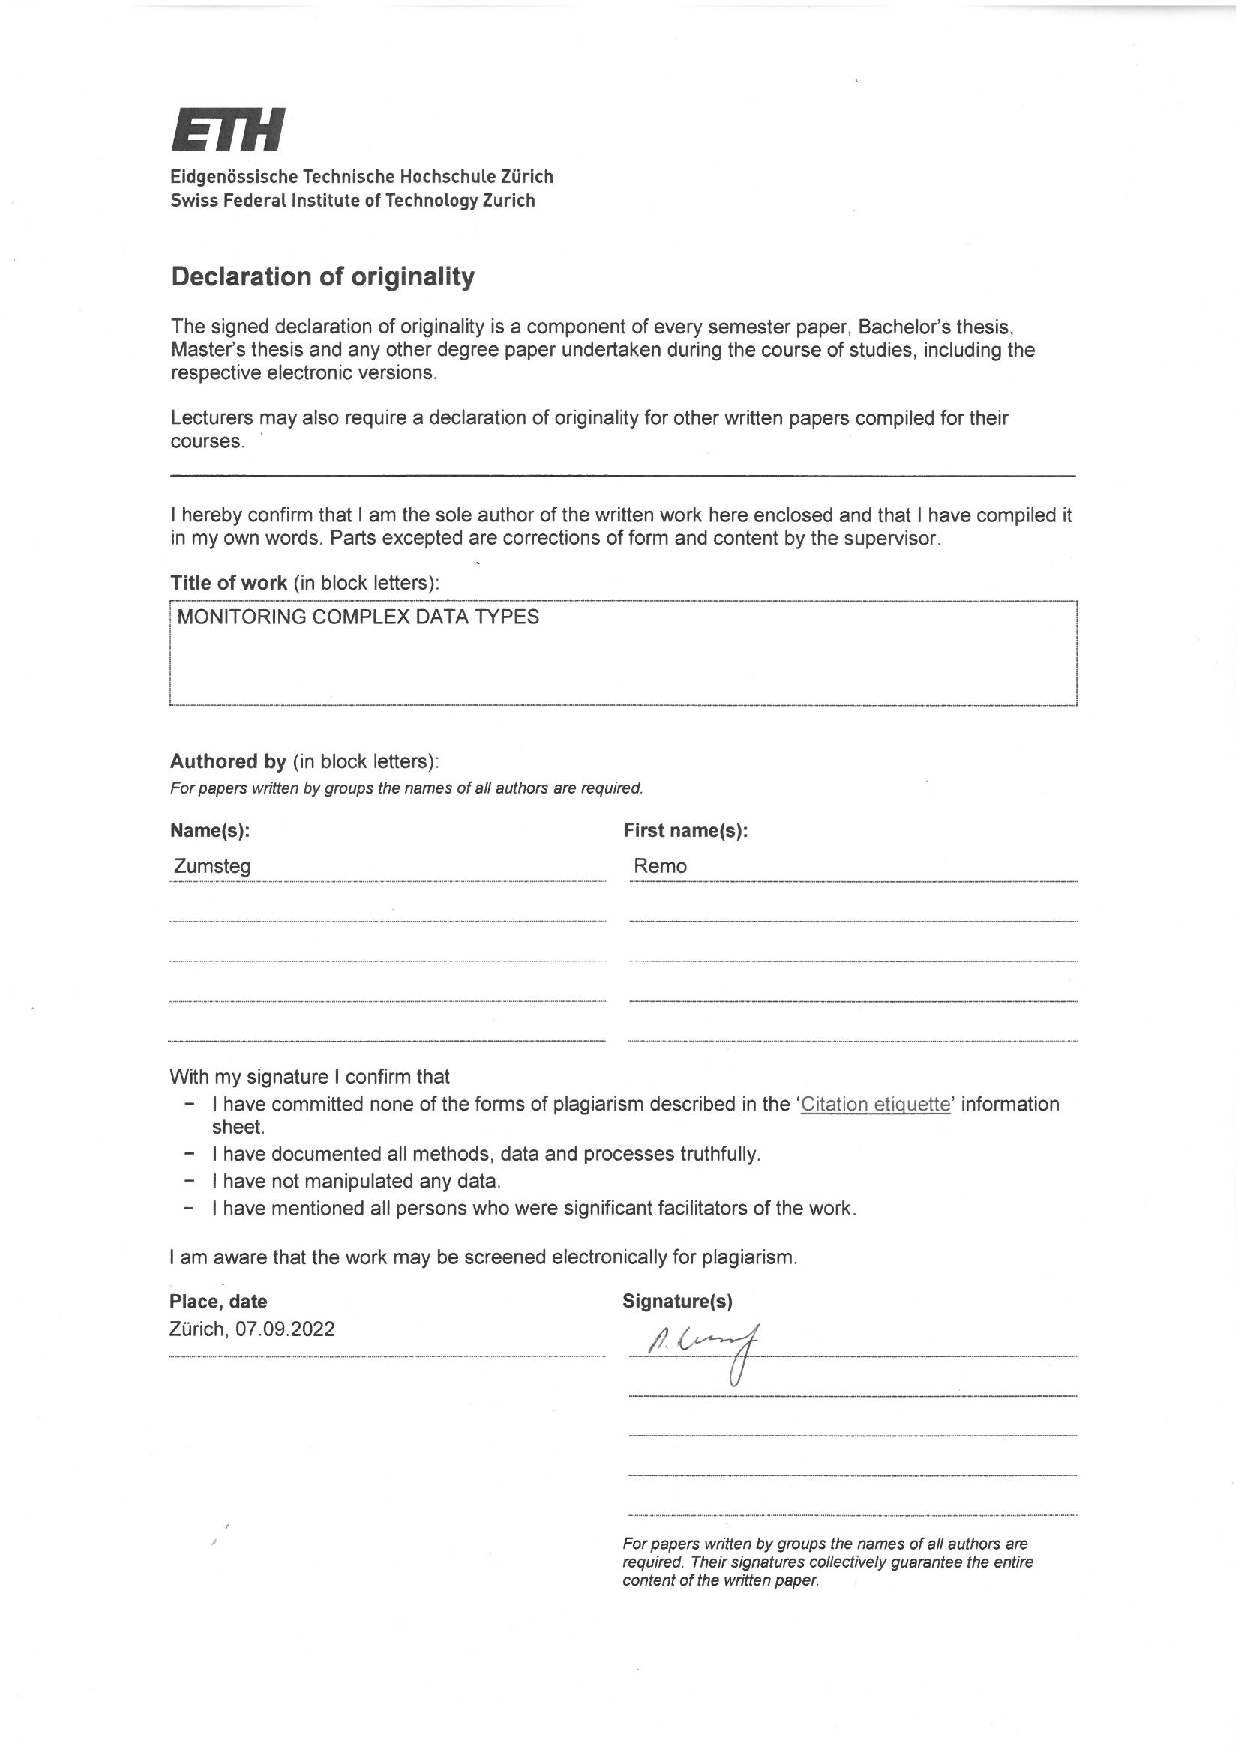
\includepdf[pages={-}]{declaration_of_originality_signed.pdf}

\end{document}
